% spellchecker: disable

\documentclass[a4paper,twoside,10.5pt]{report} %openright

\newcommand{\documenttype}{Master Thesis}
\newcommand{\thesistitle}{Deep Bayesian Neural Networks}
\newcommand{\thesissubtitle}{Subtitle}
%TODO: Substitle

\newcommand{\thesisauthor}{Søren Hartmann} % Your name :) 
\newcommand{\studentnumber}{s164182}
\newcommand{\thedate}{January, 2021} % For example "June, 2019"

\newcommand{\department}{DTU Compute}
\newcommand{\departmentdescriber}{Department of Applied Mathematics and Computer Science}
\newcommand{\addressI}{Brovej, Building 321}

%TODO: Formalia
\newcommand{\addressII}{2800 Kgs. Lyngby}
\newcommand{\departmentwebsite}{www.compute.dtu.dk}

%\usepackage{microtype}      % better looking text
%\usepackage[utf8]{inputenc}
\usepackage{fontspec}       % Package for custom fonts
\usepackage[]{geometry}     % Package for changing page margins (before fancyhdr) 
\usepackage{fancyhdr}       % Package to change header and footer
\usepackage{parskip}        % Package to tweak paragraph skipping (instead of indents a small skip is added after every paragraph)
\usepackage{titlesec}
\usepackage{tikz}           % Package for drawing
\usepackage{pgfplots}       % Package for creating graphs and charts
\usepackage{xcolor}         % Package for defining DTU colours to be used
\usepackage{amsmath}        % For aligning equations among other
\usepackage{siunitx}        % SI units
\usepackage{listings}       % Package for inserting code, (before cleveref)
\PassOptionsToPackage{hyphens}{url} % Ability to line break urls at hyphens
\usepackage{hyperref}       % Package for cross referencing (also loads url package)
\usepackage{cleveref}       % improved cross referencing
\usepackage{textcomp}       % \textdegree = °C and other useful symbols
\usepackage[english]{babel} % localisation 
\usepackage{caption}        % better captions
\usepackage{subcaption}     % for subfigures
\usepackage{csquotes}       % For biblatex with babel
\usepackage[backend=biber,style=numeric,sorting=none]{biblatex} % Package for bibliography (citing)
\bibliography{bibliography.bib}
\usepackage{tabularx}       % for ability to adjust column spacing in tabular better
\usepackage{booktabs}       % for better tables
\usepackage{float}          % floating figures in correct places
\usepackage{calc}           % Adds ability for latex to calculate (3pt+2pt) 
% \usepackage[printwatermark=false]{xwatermark} % Package for wartermark. Toggle printwatermark true or false to include or remove the watermar
\usepackage{blindtext}

\usepackage{silence}
\usepackage{lmodern}
\usepackage{charter}
% \WarningFilter{mathdesign}{Font shape}
\usepackage[charter,cal=cmcal]{mathdesign}
% \usepackage[charter]{mathdesign}

\usepackage{algorithm}
\usepackage{algpseudocode}
\usepackage{bm}
\usepackage{todonotes}
\usepackage{physics}
\usetikzlibrary{bayesnet}

\newcommand{\question}[1]{\todo[inline,color=green!20!white]{#1}}
% Colours! 
\newcommand{\targetcolourmodel}{cmyk} % rgb for a digital version, cmyk for a printed version. Only use lowercase
\selectcolormodel{\targetcolourmodel}

% Define colours from https://www.designguide.dtu.dk/
\definecolor{dtured}    {rgb/cmyk}{0.6,0,0 / 0,0.91,0.72,0.23}
\definecolor{blue}      {rgb/cmyk}{0.1843,0.2431,0.9176 / 0.88,0.76,0,0}
\definecolor{brightgreen}{rgb/cmyk}{0.1216,0.8157,0.5098 / 0.69,0,0.66,0}
\definecolor{navyblue}  {rgb/cmyk}{0.0118,0.0588,0.3098 / 1,0.9,0,0.6}
\definecolor{yellow}    {rgb/cmyk}{0.9647,0.8157,0.3019 / 0.05,0.17,0.82,0}
\definecolor{orange}    {rgb/cmyk}{0.9882,0.4627,0.2039 / 0,0.65,0.86,0}
\definecolor{pink}      {rgb/cmyk}{0.9686,0.7333,0.6941 / 0,0.35,0.26,0}
\definecolor{grey}      {rgb/cmyk}{0.8549,0.8549,0.8549 / 0,0,0,0.2}
\definecolor{red}       {rgb/cmyk}{0.9098,0.2471,0.2824 / 0,0.86,0.65,0}
\definecolor{green}     {rgb/cmyk}{0,0.5333,0.2078 / 0.89,0.05,1,0.17}
\definecolor{purple}    {rgb/cmyk}{0.4745,0.1373,0.5569 / 0.67,0.96,0,0}

\newcommand{\dtulogocolour}{white} % Colour of the DTU logo: white, black or dtured
\newcommand{\frontpagetextcolour}{white} % front page text colour: white or black
\colorlet{frontbackcolor}{blue} % Set the background colour of the front- and back page. Choose the colour so it matches the main colour of front page picture

% DTU colours for diagrams
% You might want to make the front/back page background colour the first colour in the plot cycle list.
\pgfplotscreateplotcyclelist{DTU}{%
dtured,         fill=dtured,        \\%
blue,           fill=blue,          \\%
brightgreen,    fill=brightgreen    \\%
navyblue,       fill=navyblue       \\%
yellow,         fill=yellow         \\%
orange,         fill=orange         \\%
grey,           fill=grey           \\%
red,            fill=red            \\%
green,          fill=green          \\%
purple,         fill=purple         \\%
}


% Font
% There is no corporate serif font in the DTU design guide. The DTU design team has proposed to use Neo Sans for headings - and Arial for the body text.
% To change heading font to NeoSans Pro please upload both NeoSansPro-Regular.otf and NeoSansPro-Medium.otf to the root directory.
\setmainfont{Arial}
\renewcommand\thepart{Part \Roman{part}}
\IfFontExistsTF{NeoSansPro-Medium.otf}
{ %If True set headings to NeoSans Pro
\newfontface\NeoSansProReg{NeoSansPro-Regular.otf}
\newfontface\NeoSansProMed{NeoSansPro-Medium.otf}
\titleformat{\part}[display]{\NeoSansProMed \huge \centering}{\NeoSansProMed \Huge \thepart}{1em}{\thispagestyle{empty}}{}
\titleformat{\chapter}{\NeoSansProMed\huge}{\thechapter}{1em}{\raggedright}
\titleformat{\section}{\NeoSansProMed\Large}{\thesection}{1em}{\raggedright}
\titleformat{\subsection}{\NeoSansProMed\large}{\thesubsection}{1em}{\raggedright}
\titleformat{\subsubsection}{\NeoSansProMed\normalsize}{\thesubsubsection}{1em}{\raggedright}
\newcommand\TitleFont[1]{{\NeoSansProMed #1}}
\newcommand\titlefont[1]{{\NeoSansProReg #1}}
}
{ % If false
\titleformat{\part}[display]{\bfseries\huge \centering}{\bfseries\Huge \thepart}{1em}{\thispagestyle{empty}}{}
\titleformat{\chapter}{\bfseries\huge}{\thechapter}{1em}{\raggedright}
\titleformat{\section}{\bfseries\Large}{\thesection}{1em}{\raggedright}
\titleformat{\subsection}{\bfseries\large}{\thesubsection}{1em}{\raggedright}
\titleformat{\subsubsection}{\bfseries\normalsize}{\thesubsubsection}{1em}{\raggedright}
\newcommand\TitleFont[1]{{\bfseries #1}}
\newcommand\titlefont[1]{{#1}}
}
\urlstyle{sf}
%\def\UrlFont{\NeoSansProReg}


% If you wish to use the pdflatex compiler, sans-serif Helvetica can be used as a replacement for Arial. In this way you will be able to use the microtype package. Remember to add \usepackage[utf8]{inputenc} and disable the fontspec package. 
%\newcommand\TitleFont[1]{{\bfseries #1}}
%\newcommand\titlefont[1]{{#1}}
%\fontfamily{qhv}\selectfont
%\renewcommand{\familydefault}{\sfdefault}


% Watermark for confidential or draft (or anything else)
%\sffamily % set the correct font for the watermark
\newsavebox\mybox
\savebox\mybox{\tikz[color=grey,opacity=0.5]\node{Template};}

\newwatermark*[
  oddpages,
  angle=60,
  scale=12,
  %fontfamily=qhv,
  xpos=-40,
  ypos=30,
]{\usebox\mybox}

\newwatermark*[
  evenpages,
  angle=60,
  scale=12,
  %fontfamily=qhv,
  xpos=-50,
  ypos=30,
]{\usebox\mybox}


% Table of contents (TOC) and numbering of headings
\setcounter{tocdepth}{1}    % Depth of table of content: sub sections will not be included in table of contents
\setcounter{secnumdepth}{2} % Depth of section numbering: sub sub sections are not numbered

\makeatletter % Reset chapter numbering for each part
\@addtoreset{chapter}{part}
\makeatother  

% Spacing of titles and captions
\titlespacing\chapter{0pt}{0pt plus 4pt minus 2pt}{4pt plus 2pt minus 2pt}
\titlespacing\section{0pt}{12pt plus 3pt minus 3pt}{2pt plus 1pt minus 1pt}
\titlespacing\subsection{0pt}{8pt plus 2pt minus 2pt}{0pt plus 1pt minus 1pt}
\titlespacing\subsubsection{0pt}{4pt plus 1pt minus 1pt}{-2pt plus 1pt minus 1pt}
\captionsetup{belowskip=\parskip,aboveskip=4pt plus 1pt minus 1pt}

% Setup header and footer
\fancypagestyle{main}{% All normal pages
    \fancyhead{}
    \fancyfoot{}
    \renewcommand{\headrulewidth}{0pt}
    \fancyfoot[LE,RO]{\footnotesize \thepage}
    \fancyfoot[RE,LO]{\footnotesize \thesistitle} % - \rightmark
    \fancyhfoffset[E,O]{0pt}
}
\fancypagestyle{plain}{% Chapter pages
    \fancyhead{}
    \fancyfoot{}
    \renewcommand{\headrulewidth}{0pt}
    \fancyfoot[LE,RO]{\footnotesize \thepage}
    \fancyfoot[RE,LO]{\footnotesize \thesistitle} % - \leftmark
    \fancyhfoffset[E,O]{0pt}
}


% Setup for diagrams and graphs (tikz pictures) 
\usetikzlibrary{spy}    % For magnifying anything within a tikzpicture, see the line graph
\usepgfplotslibrary{statistics} % Package for the boxplot
\pgfplotsset{ % Setup for diagrams
compat=newest,
major x grid style={line width=0.5pt,draw=grey},
major y grid style={line width=0.5pt,draw=grey},
legend style={at={(0.5,-0.1)}, anchor=north,fill=none,draw=none,legend columns=-1,/tikz/every even column/.append style={column sep=10pt}},
axis line style={draw=none},
tick style={draw=none},
every axis/.append style={ultra thick},
tick label style={/pgf/number format/assume math mode}, % To apply main font to tick labels (numbers on the axis)
}
\tikzset{every mark/.append style={scale=1.5}}


% Hypersetup
\hypersetup{
    pdfauthor={\thesisauthor},
    pdftitle={\thesistitle},
    pdfsubject={\thesissubtitle},
    pdfdisplaydoctitle,
    bookmarksnumbered=true,
    bookmarksopen,
    breaklinks,
    linktoc=all,
    plainpages=false,
    unicode=true,
    colorlinks=false,
    hidelinks,                        % Do not show boxes or coloured links.
}


% Listings setup
\lstset{
    basicstyle=\footnotesize\ttfamily,% the size of the fonts that are used for the code
    commentstyle=\color{green},       % comment style
    keywordstyle=\bfseries\ttfamily\color{blue}, % keyword style
    numberstyle=\sffamily\tiny\color{grey}, % the style that is used for the line-numbers
    stringstyle=\color{purple},       % string literal style
    rulecolor=\color{grey},           % if not set, the frame-color may be changed on line-breaks within not-black text (e.g. comments (green here))
    breakatwhitespace=false,          % sets if automatic breaks should only happen at whitespace
    breaklines=true,                  % sets automatic line breaking
    captionpos=b,                     % sets the caption-position to bottom
    deletekeywords={},                % if you want to delete keywords from the given language
    escapeinside={\%*}{*)},           % if you want to add LaTeX within your code
    frame=single,                     % adds a frame around the code
    xleftmargin=4pt, 
    morekeywords={*,...},             % if you want to add more keywords to the set
    numbers=left,                     % where to put the line-numbers; possible values are (none, left, right)
    numbersep=10pt,                   % how far the line-numbers are from the code
    showspaces=false,                 % show spaces everywhere adding particular underscores; it overrides 'showstringspaces'
    showstringspaces=false,           % underline spaces within strings only
    showtabs=false,                   % show tabs within strings adding particular underscores
    stepnumber=1,                     % the step between two line-numbers. If it's 1, each line will be numbered
    tabsize=2,                        % sets default tabsize to 2 spaces
    title=\lstname,                   % show the filename of files included with \lstinputlisting; also try caption instead of title
}

% Signature field
\newlength{\myl}
\newcommand{\namesigdatehrule}[1]{\par\tikz \draw [black, densely dotted, very thick] (0.04,0) -- (#1,0);\par}
\newcommand{\namesigdate}[2][]{%
\settowidth{\myl}{#2}
\setlength{\myl}{\myl+10pt}
\begin{minipage}{\myl}%
\begin{center}
    #2  % Insert name from the command eg. \namesigdate{\authorname}
    \vspace{1.5cm} % Spacing between name and signature line 
    \namesigdatehrule{\myl}\smallskip % Signature line and a small skip
    \small \textit{Signature} % Text under the signature line "Signature"
    \vspace{1.0cm} % Spacing between "Signature" and the date line
    \namesigdatehrule{\myl}\smallskip % Date line and a small skip
    \small \textit{Date} % Text under date line "Date" 
\end{center}
\end{minipage}
}

% For the back page: cleartoleftpage
\newcommand*\cleartoleftpage{%
  \clearpage
  \ifodd\value{page}\hbox{}\newpage\fi
}


\begin{document}

\pagenumbering{roman}
\title{\thesistitle} 
\author{\thesisauthor} 
\date{\thedate} 

\begin{titlepage}

\newgeometry{left=11mm,right=11mm,top=50mm,bottom=0pt}
\pagecolor{frontbackcolor}
\color{\frontpagetextcolour}

{ % Thesis title (to change see Setup/Settings.tex) 
\Huge
\begin{tabular}{p{\linewidth}}
\TitleFont{\thesistitle}   \\ 
\TitleFont{\thesissubtitle} \bigskip \\ 
\titlefont{\documenttype}
\end{tabular}
}

% DTU department (to change see Setup/Settings.tex) 
\begin{tikzpicture}[remember picture,overlay]
\node[anchor=north east, 
      xshift=-10mm, 
      yshift=-12mm] 
      at (current page.north east) 
      {
        \color{\frontpagetextcolour}
        \begin{tabular}{r} 
        \textbf{\department} \\ 
        \departmentdescriber
        \end{tabular}
      }; 
\end{tikzpicture}
%TODO: Forside  

% DTU logo
\begin{tikzpicture}[remember picture,overlay]
\node[anchor=north west, 
      xshift=8.9mm, 
      yshift=-8.3mm] 
     at (current page.north west) 
     {\includegraphics[width=14.75mm,keepaspectratio]{Pictures/Logos/\dtulogocolour_\targetcolourmodel.pdf}}; 
\end{tikzpicture}

% Cover photo
\begin{tikzpicture}[remember picture,overlay]
\node[anchor=south, % anchor is bottom of picture
      xshift=0pt, 
      yshift=-2.9mm] % shifting picture to actually be at the bottom of the page
     at (current page.south) % placement at bottom of the page
     {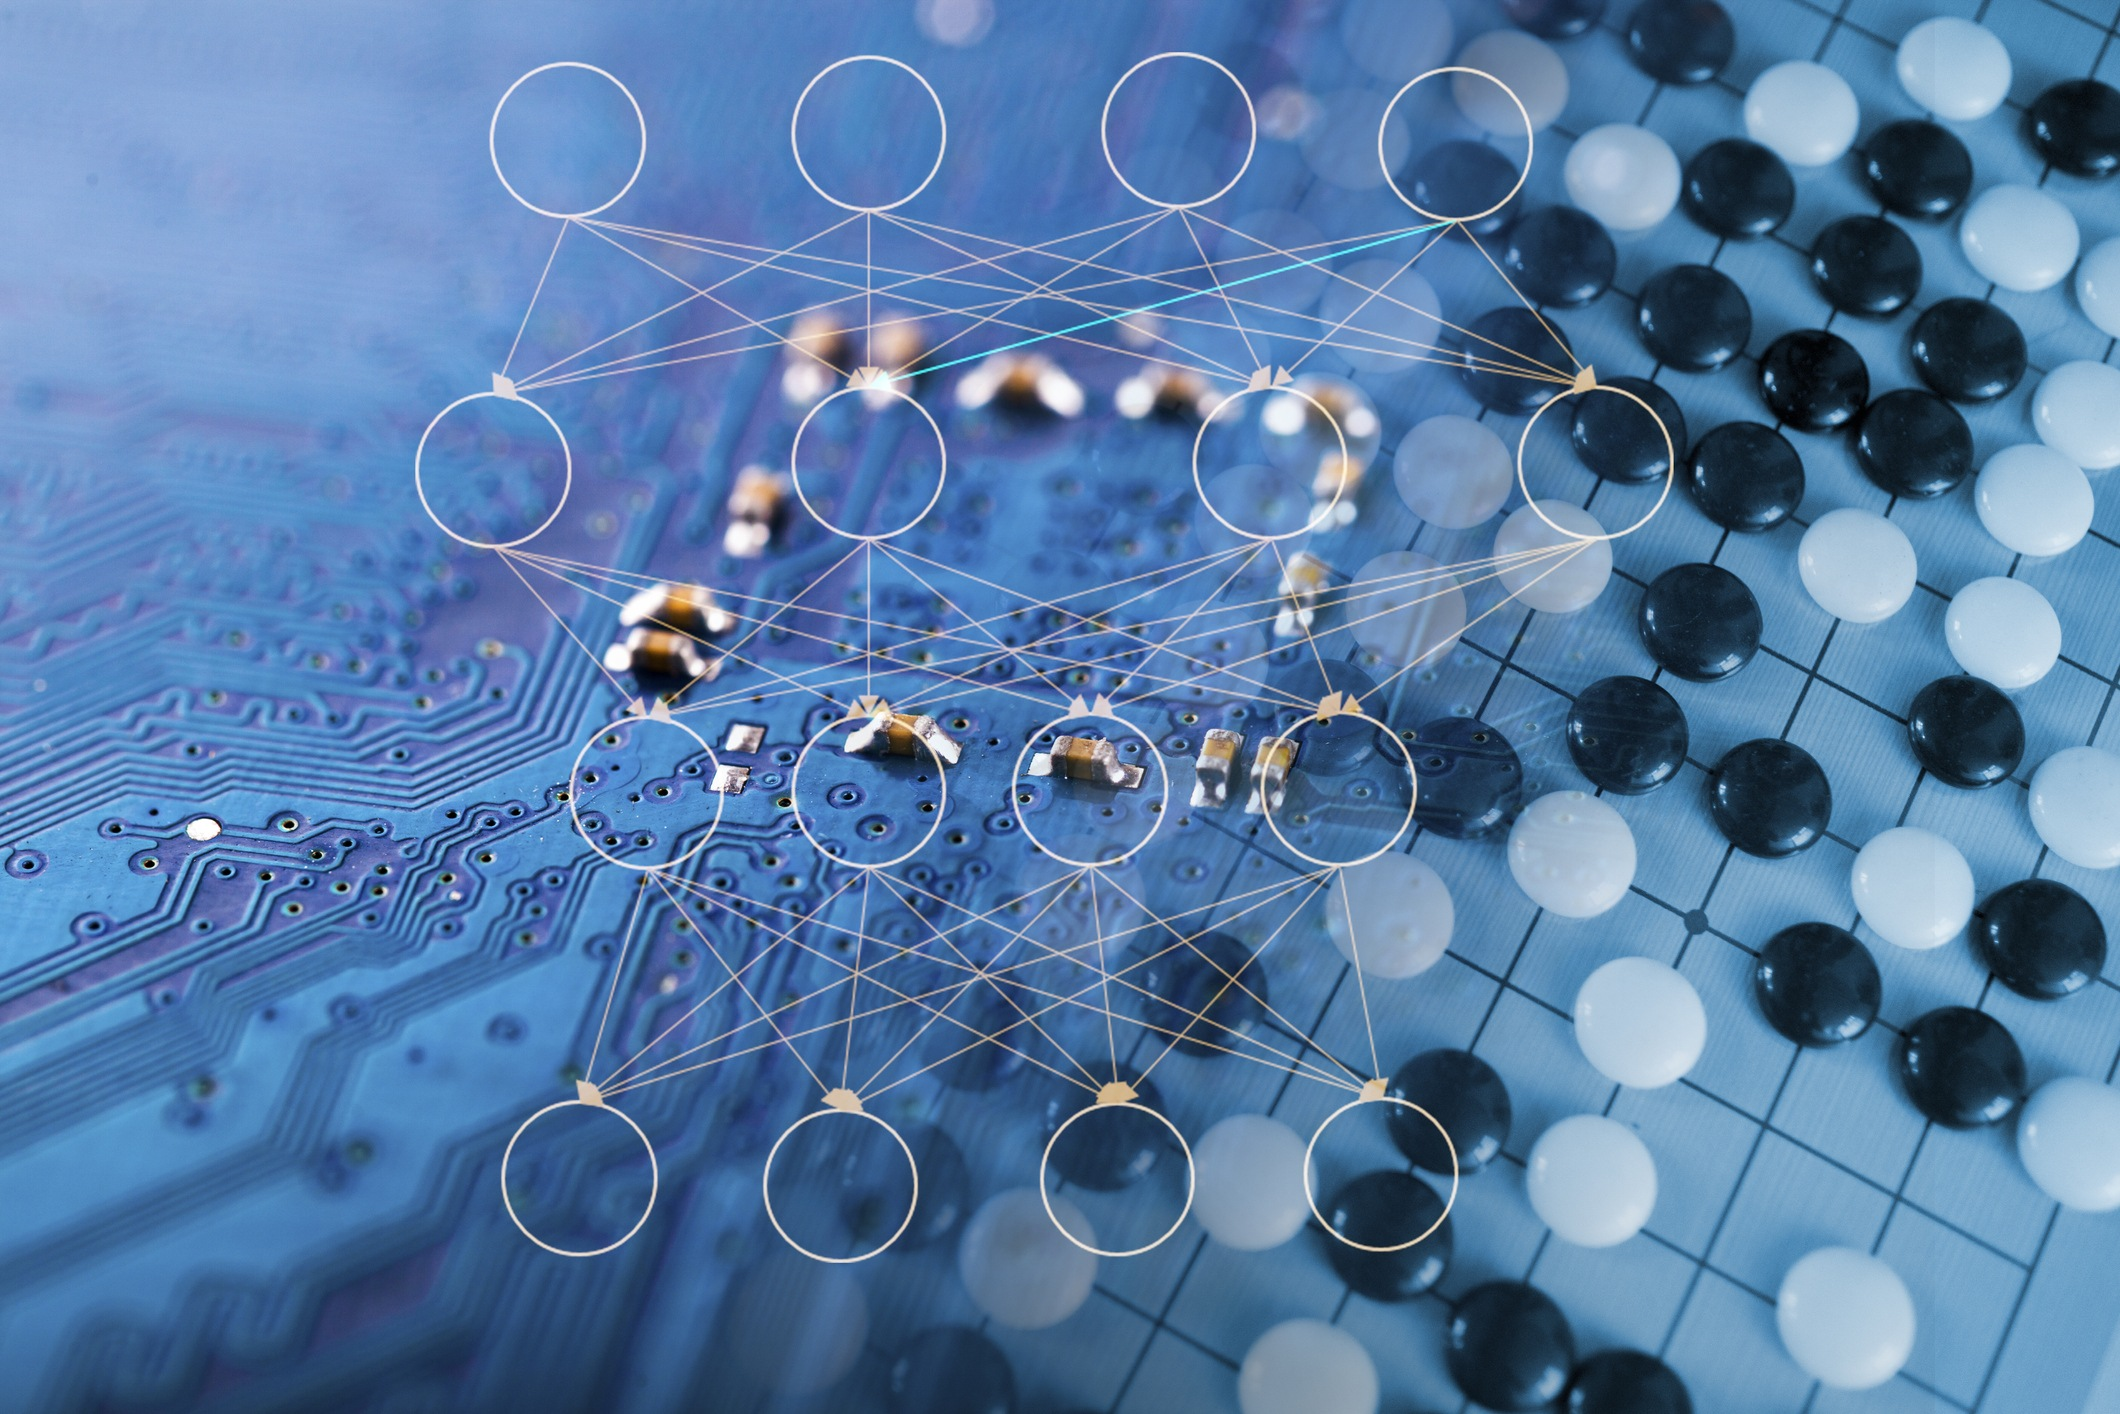
\includegraphics[height=18.9cm,keepaspectratio]{Pictures/deep-learning-stock.jpg}};
\end{tikzpicture}




\end{titlepage}

\pagecolor{white}
\newgeometry{top=2.81cm, bottom=2.75cm, outer=2.5cm, inner=3.5cm}
\pagestyle{empty}
\cleardoublepage 
\thispagestyle{empty}
\setcounter{page}{1}
\vspace*{\fill}

\textbf{\thesistitle} \newline
\thesissubtitle

\smallskip

\documenttype \newline
\thedate

\smallskip

By \newline
\thesisauthor

\bigskip

\begin{tabularx}{\textwidth}{@{}lX@{}}
    Copyright: & Reproduction of this publication in whole or in part must include the customary bibliographic citation, including author attribution, report title, etc. \\
    Cover photo: & Vibeke Hempler, 2012 \\
    Published by: & DTU, \departmentdescriber, \addressI, \addressII ~Denmark  \\
     & \url{\departmentwebsite} \\
    ISSN: & [0000-0000] (electronic version) \\
    ISBN: & [000-00-0000-000-0] (electronic version) \\
    & \\
    ISSN: & [0000-0000] (printed version) \\
    ISBN: & [000-00-0000-000-0] (printed version)
\end{tabularx}



\clearpage 
\pagestyle{main}
\section*{Approval}
\addcontentsline{toc}{section}{Preface}

This Master's thesis was prepared at the Department of Applied Mathematics and Computer Science at the Technical University of Denmark in fulfillment of the requirements for the degree Master of Science in Engineering, MSc Eng, in Mathematical Modeling and Computation.


\vfill

\begin{center}
\namesigdate{\thesisauthor~-~\studentnumber}
\end{center}

\vfill


\clearpage 
\section*{Abstract}
\addcontentsline{toc}{section}{Abstract}

intro

teori

We implement both of these approaches using the PyTorch and PyTorch Lightning frameworks.

We implement two different approaches, the first being a Markov chain Monte Carlo algorithm, SGHMC introduced in \cite*{chen_stochastic_2014}.
This algorithm is a variation of the Hamiltonian Monte Carlo algorithm, allowing for sampling in a batched learning environment.
SGHMC accomplishes this by modifying the stochastic dynamic to correct for the additional variance by introducing a friction term. 
This approach works well in small-scale simulated experiments. 
We also find that introducing a gradient variance estimator for these simulated scenarios can improve the performance of the sampling algorithm.
The second approach is approximating the Bayesian posterior using the variational inference algorithm.

hurtig konklu

% \blindtext






\clearpage 
\section*{Acknowledgements}
\addcontentsline{toc}{section}{Acknowledgements}

\blindtext[2]
\cleardoublepage 


\tableofcontents
\cleardoublepage 

%%%%%%%%%%%%%%%%%%%%%%%%%%%%%%%%%%%%%%%%%%%%%%%%%%%%%%%
\pagenumbering{arabic}
\chapter{Introduction}
In every sense of the word, modern machine learning models are unbelievable. 
Following our increase in computational resources, we can construct and train ever-more powerful and expressive models.
Combined with the use of massive datasets, these models are changing the world around us for better or for worse. 
At the same time, we are also finding it increasingly difficult to reason about how the models interpret and reason about the world.

For instance, we see that as models are achieving better performance, they also become increasingly poorly calibrated\autocite{guo_calibration_2017}, making us question how much trust we should put in predictions made by the models. 
We also see examples of specific adversarial attacks, for which even powerful models completely break down \autocite{fezza_perceptual_2019}.
Issues such as these warrant consideration, especially in areas where the robustness of models is paramount, be these medical applications or self-driving cars.

Therefore, we are motivated to seek techniques and interpretations to achieve more robust and preferably better-performing models.

We can generally frame the most common machine learning problems as the task of predicting an output value given an input value. 
We can often formulate these predictions as a conditional probability of some output targets given some input data.
Typically, we parameterize this model using some parameters that are often unknown.
These models are made very flexible by defining them using many parameters, enabling them to account for complex structures in the data. 

Training these models is usually viewed as an optimization problem, figuring out values of the model parameters that minimize some objective function.
We thus typically end up relying on the parameter estimates being robust. 

In opposition to this frequentist approach, a Bayesian approach usually seeks to integrate our uncertainty about the parameters instead of relying on point estimates of the unknown parameters.

Using this method, we can generally achieve more robust results than just using point estimates, at least for simple models.
However, if we are to apply this method to deep learning models, we are faced with some difficulties due to the large amounts of data and the high number of parameters.

Bayesian Neural Networks have been the subject of some interest and several papers over the recent years. 
In \autocite{chen_stochastic_2014} the Hamiltonian Monte Carlo algorithm for Bayesian inference is adapted to use in a batched learning setting. 
In \autocite{blundell_weight_2015} they use a variational distribution is used for approximating the posterior, allowing for an optimization-based approach of achieving approximate Bayesian inference.

This project explores implementing and applying the ideas from these two papers.
First, we will walk through and describe the two approaches, including the mathematical results underpinning them.
We then compare the probabilistic methods with each other and a frequentist baseline.
Along the way, we will explore whether we can implement Bayesian methods as a drop-in replacement for frequentist methods.
\chapter{Inference}

Data is $\mathcal{D} = (\bm{X}, \bm{Y})$, where $\bm{X} = (x_1,\dots,x_N)$ are covariates and $\bm{Y} = (y_1, \dots, y_N)$ are attributes we want to model.
Given new data $x^\ast$, find the predictive distribution $p(y^\ast | x^\ast)$ 

Marginalize out the parameters of the model, $\theta$.
\begin{align*}
    p(y^\ast | x^\ast) &= E_{p(\theta|\mathcal{D})} p(y^\ast | x^\ast, \theta) \\
                       &= \int_{\theta} p(y^\ast | x^\ast, \theta)  p(\theta|\mathcal{D}) d\theta
\end{align*}
In practice, at least in the case of deep learning models, the integral of the expectation feasable to evalutate exactly. 
We therefore resort to approximate methods, such as the Monte Carlo estimate:
\begin{align*}
    p(y^\ast | x^\ast)  \approx \frac{1}{N} \sum_{j=1}^N p(y^\ast | x^\ast, \theta^{(i)}) 
\end{align*}
Where $\theta^{(i)}$ are samples from the posterior distribution:
\begin{align*}
    p(\theta | \mathcal{D}) 
    &= p(\theta | \bm{X}, \bm{Y}) \\
    &= \frac{p(\bm{Y} |\theta, \bm{X}) p(\theta|\bm{X})}{p(\bm{Y}) } \\
    &= \frac
    {\left(\prod_{i=1}^N p(y_i |\theta, x_i)\right) p(\theta)}
    {p(\bm{Y}) }  
\end{align*}
The unconditional  observation model, $p(y)$, is also not easily evalutated. 
In the following, we will discuss two different strategies to get around this. 
The first is to use sampling methods that only requires the sampling distribution $f(\theta)$ up to a constant factor $\hat{f}(\theta)\propto f(\theta)$. 
This is useful since 
\begin{align*}
    p(\theta | \mathcal{D}) 
    &= \frac
    {\left(\prod_{i=1}^N p(y_i |\theta, x_i)\right) p(\theta)}
    {p(\bm{Y}) }  \\
    &\propto \left(\prod_{i=1}^N p(y_i |\theta, x_i)\right) p(\theta)
\end{align*}
and both the likelihood, $p(y_i |\theta, x_i)$ and the prior $p(\theta)$ are specified as part of the graphical model, at least up to a constant factor. 
The other approach is to use an approximate posterior $q(\theta)$ in place of the exact posterior. 

The different methods are applicable not only for sampling from a posterior $p(\theta | \mathcal{D})$, but from sampling from any random variable with a density function $p(x)$ speficied up to a constant factor.

\section{Markov Chain Monte Carlo}
Suppose we want to sample from a target distribution $p(x)$, yet we only know $\tilde{p}(x) = 1/K\cdot p(x)$, where $K$ is constant in $x$.
The Markov Chain Monte Carlo (MCMC) methods use a Markov chain with transition to generate samples sequentially from $p(x)$. 
We achieve this by ensuring that the Markov chain with transition density $q(x^\prime | x)$ satisfies two requirements

\begin{itemize}
    \item The target distribution $p(x)$ stationary with respect to the Markov chain, that is:
    \begin{align} \label{eq:stationarity}
        p(x^\prime) = \int_{\Omega} q(x^\prime| x) p(x) \dd{x} 
    \end{align}
    \item The Markov chain eventually reaches the stationary distribution $p(x)$. This is satisfied by ensuring the markov chain is irreducible and aperiodic.

\end{itemize}
A sufficent criteria for $p(x)$ to be stationary with respect to the Markov chain is that the transition probablities $q(x^\prime|x)$ satisfy the property of detailed balance:
\begin{align*}
    p(x)q(x^\prime | x) = p(x^\prime)q(x| x^\prime).
\end{align*}
This implies stationary since
\begin{align*}
    \int_{\Omega} q(x^\prime | x) p(x) \dd{x} 
    &= \int_{\Omega}  p(x^\prime)q(x| x^\prime) \dd{x} \\ 
    &=  p(x^\prime) \int_{\Omega} q(x| x^\prime) \dd{x} \\
    &=  p(x^\prime) \cdot 1 \\
    &= p(x^\prime).
\end{align*}

The following chapters discusses a straigh forward method applying the property of detailed balance.

\subsection{Metropolis-Hastings}

Suppose at some step $t$, the Markov chain has state $x^{(t)}$. The Metropolis-Hastings algorithm uses a symmetric proposal distribution $g(x|x^{(t)})$ to generate a new sample, $x^\prime$. The sample is then \emph{accepted} with probability:
\begin{align*}
    A(x^{\prime}, x^{(t)}) = \min\left\{1, \frac{\tilde{p}(x^\prime)}{\tilde{p}(x^{(t)})}\right\}
\end{align*}
If the sample is accepted, $x^{(t+1)} \gets x^\prime$. Otherwise, the new state is rejected and $x^{(t+1)} \gets x^{(t)}$. This process is then repeated until we have obtained the required amount of samples $x^{(1)},\dots,x^{(N)}$. 


The transition density $q(x_{k+1}|x_k)$ is such that 
\begin{align}
    P(x_{k+1} \in B | x_k ) = \int_B q (x_{k+1}|x_k )\dd x_{k+1}
\end{align}

Using the proposal distribution we generate a sample $x^\ast_{k+1}$.The next sample $x_{k+1}$ is then within some $B\subset \Omega$, if and only if $x^\ast_{k+1}\in A$ and the sample is accepted, ie.
\begin{equation}
    \begin{aligned}
        P(x_{k+1} \in B | x_k ) 
        &= \int_\Omega P( x_{k+1} \in B | x^\ast_{k+1},x_k) g(x^\ast_{k+1}|x_k) \dd{x^\ast_{k+1}}\\
        &= \int_B P( x_{k+1} \in B | x^\ast_{k+1},x_k) g(x^\ast_{k+1}|x_k) \dd{x^\ast_{k+1}} \\
        &= \int_B A(x^\ast_{k+1}, x_k) g(x^\ast_{k+1}|x_k) \dd{x^\ast_{k+1}}
    \end{aligned}
\end{equation}
We thus see that the transition density of this sampling scheme is
\begin{align}
    q(x^\prime|x) = g(x^\prime | x) A(x^\prime, x)
\end{align} 
Suppose at some point, the state of the chain is $x$. The transition density to some other state $x^\prime$ is then:
\begin{align*}
    q(x^\prime|x) = g(x^\prime | x) A(x^\prime, x)
\end{align*}
We can verify that this transition probability does indeed satisfy the property of detailed balance:
\begin{align*}
    p(x)q(x^\prime|x) &= p(x)g(x^\prime | x) A(x^\prime, x) \\
                      &= p(x)g(x^\prime | x) \min\left\{1,  \tilde{p}(x^\prime) / \tilde{p}(x)\right\} \\
                      &= \underbrace{p(x)}_{\geq 0} \underbrace{g(x^\prime | x)}_{=g(x | x^\prime)} \min\left\{1,  p(x^\prime) / p(x)\right\} \\
                      &= g(x | x^\prime) \min\left\{p(x), p(x^\prime)\right\} \\
                      &= g(x | x^\prime) p(x^\prime) \min\left\{p(x)/p(x^\prime), 1\right\} \\
                      &= p(x^\prime) g(x | x^\prime)  A(x ,x^\prime) = p(x^\prime) q(x|x^\prime).
\end{align*}
Thus, the Markov chain satisfies the property of detailed balance, and is stationary with respect to the Markov chain. If we choose our proposal distribution such that the chain is also irreducible and aperiodic, eg. by having $q(x^\prime|x) \neq 0$ for all $x^\prime,x$, the sample distribution should therefore eventually converge towards $p(x)$. 

While the Metropolis-Hastings algorithm will eventually sample from the correct distribution, it is not given that this necessarily occurs within a reasonable time. 
We are essentially hoping that our proposal distribution $g(x^\prime | x)$ reliably doesn't propose new states $x^\prime$ with much lower probability, $p(x^\prime) \ll p(x) $, in order to keep the acceptance probability $A(x^\prime, x)$ at reasonable levels. 
For simple problems, this can often be done by tuning a Gaussian distribution around the current state, however for problems with high dimensionality and complex target distributions, this strategy may fall short.

\subsection{Gibbs sampling}

Suppose we had some way of easily sampling each of our variables conditioned on our other variables, that is $p(x_i|\bm{x}_{\setminus i})$. 
The Gibbs sampling strategy generates a new sample $\bm{x}$ by sampling each variable $x_i$ in turn from $p(x_i|\bm{x}_{\setminus i})$.  
First we need to show that the joint distribution $p(\bm{x})$ is invariant to each of these steps. 
In order to argue for the stationarity of this procedure, we argue that each of the steps is invariant to the target distribution.

The transition density $q(x^\prime| x)$ can be specified using the Dirac Delta function as:
\begin{align*}
    q(x^\prime| x) = \delta_{x_{\setminus i}}(x^\prime_{\setminus i}) p(x_i^\prime|x_{\setminus i})
\end{align*}

We can verify that this transition density does inseed satisfy the stationarity requirements in \cref{eq:stationarity}.
\begin{align*}
    \int_{\Omega} q(x^\prime| x) p(x) \dd{x}  
    &= \int_{\Omega}  \delta_{x_{\setminus i}}(x^\prime_{\setminus i}) p(x_i^\prime|x_{\setminus i}) p(x_i,x_{\setminus i}) \dd{x_{\setminus i}} \dd{x_i} \\
    &= \int_{\Omega} p(x^\prime_i|x^\prime_{\setminus i}) p(x_i,x^\prime_{\setminus i}) \dd{x_i} \\ 
    &= p(x^\prime_i|x^\prime_{\setminus i}) \int_{\Omega}  p(x_i,x^\prime_{\setminus i}) \dd{x_i} \\ 
    &= p(x^\prime_i|x^\prime_{\setminus i}) \int_{\Omega}  p(x_i | x^\prime_{\setminus i}) p(x^\prime_{\setminus i}) \dd{x_i} \\ 
    &= p(x^\prime_i|x^\prime_{\setminus i}) p(x^\prime_{\setminus i}) \int_{\Omega}  p(x_i | x^\prime_{\setminus i})  \dd{x_i} \\ 
    &= p(x^\prime_i|x^\prime_{\setminus i}) p(x^\prime_{\setminus i}) \cdot 1 \\
    &=  p(x^\prime_i,x^\prime_{\setminus i})  \\
    &= p(x^\prime)
\end{align*}

If the condtional distributions $p(x_i|x_{\setminus i})$ are non-zero for all values of all variables $x_i$, the chain is also ergodic. If not, as discussed in \cite{bishop_pattern_2006}, ergodicity of the sampling strategy will have to be proven explicitly.

\subsection{Hamiltonian Monte Carlo}

A popular method to improve the proposal strategy is the Hamiltonian Monte Carlo (HMC) algorithm. 
From the Metropolis-Hastings algorithm we see that we need a proposal strategy, that both leaves the target distribution invariants and while being able to take as large steps as possible in order to explore the parameter space.
Borrowing from the field of dynamical systems, HMC uses the notion of conservation of kinetic and potential energy to generate samples from the target distribution. 
Specifically, the variables are modelled as an Hamiltonian system. To this end, we define the \emph{momentum}, $r_i$ of each variable $x_i$.
\begin{align*}
    \dv{x_i}{t} = M^{-1} r_i
\end{align*}
Where $M$ is the mass matrix of the system. Then the kinetic energy, $K$ of the particle can be described as a function of the momentum:
\begin{align*}
    K(r) = \frac{1}{2}r^T M^{-1} r.
\end{align*}
The rate of change of the momentum, ie. the acceleration is given by the negative gradient of the potential energy, $E$:
\begin{align*}
    \dv{r_i}{t} = -\pdv{E(x)}{x_i}
\end{align*}
Introducing the Hamiltonian function $H(x, r) = K(r) + E(x)$, we can write the dynamics governing the system as
\begin{equation}\label{eq:hmc-dynamics}
    \begin{aligned}
        \dv{x_i}{t} &= \phantom{-}\pdv{H}{r_i}\\
        \dv{r_i}{t} &= -\pdv{H}{x_i}
    \end{aligned}
\end{equation}
Since $\pdv{H}{r_i} = \pdv{K}{r_i} = M^{-1}r_i$ and $-\pdv{H}{x} = -\pdv{E}{x_i}$. 
Such a system is called a Hamiltonian system, and the useful property that values of $H$ remain constant along trajectories of the system.
We then consider sampling from the joint density:
\begin{align} \label{eq:hmc-joint}
    p(x, r) = \frac{1}{C_H} \exp\left[ -H(x, r)\right] = \frac{1}{C_H} \exp\left[-K(r) - E(x)  \right].
\end{align}
If we throw away the samples from $r$, we are then left with samples from the marginal distribution of $x$. If we then introduce the negative log density as potential energy of the particle,
\begin{align*}
    E(x) = -\log{p(x)}
\end{align*}
looking at \cref{eq:hmc-joint}, we see that under the distribution $p(x, r)$, the variables $x$ and $r$ are independent, and the marginal distribution of $x$ indeed factors out to be the target distribution $p(x)$. 

\newcommand{\newx}{x^{\prime}}
\newcommand{\newr}{{r^{\prime}}}
\newcommand{\oldx}{{x^{(k)}}}
\newcommand{\oldr}{{r^{(k)}}}
\newcommand{\nextx}{x^{(k+1)}}
\newcommand{\nextr}{{r^{(k+1)}}}

Ideally we would sample from $p(x, r)$ in two steps. Suppose the current position in phase space is $(\oldx, \oldr)$. 
First, the momentum is resampled as $\oldr^\ast\sim \mathcal{N}(0, M^{-1})$. Then, the dynamics of the system is simulated for some amount of time $\Delta$ to yield the next sample $(\nextx, \nextr) =\phi_\Delta(\oldx, \oldr^\ast)$.
% Let $\phi(x, r, t):$ be the dynamical system defined in \cref{eq:hmc-dynamics}, 

The stationarity of this procedure is shown by showing the stationarity of each of the two steps. From \cref{eq:hmc-joint}, we see that $p(r|x) \propto \exp[-K(r)] = \exp[\frac{1}{2}r^tM^{-1}r]$, ie. the conditional distribution of $r$ is $\mathcal{N}(0, M^{-1})$.
By resampling the momentum, we are thus performing a Gibbs step, and as seen previously, this does indeed have $p(x, y)$ as stationary distribution.
\question{$\delta(z-a)$ vs $\delta_a(z)$? Nemmere måde at vise det på?}
Then, since we are deterministically simulating the system, we can model the next transition density using the delta function, $q(z^\prime|z) = \delta(z^\prime - \phi_\Delta(z))$, where $z=(x, r)$. 
Since $H$ is constant along trajectories of the system, $p(z) =p(\phi_t(z))$ for any $t$, and thus
\begin{align} \label{eq:}
    \int_{\Omega} q(z^\prime| z ) p(z) \dd{z} = \int_{\Omega} \delta(z^\prime - \phi_\Delta(z))p(z) \dd{z} 
    = p(\phi_{-\Delta}(z^\prime)) = p(z^\prime).
\end{align}
The second step therefore also satisfies the stationarity requirement. The ergodicity of the sampling procedure is ensured by the initial resampling of the procedure. Since we are sampling the momentum from a normal distribution, there is a non zero probablity of reaching any point in phase space for each sample.

In practice, it is not possible to exactly simulate the system, and we therefore make use of a leapfrog integrator, $\hat{\phi}_\epsilon^T$, simulating the dynamics using $T$ discrete time steps of size $\epsilon$. While we can obtain very good approximations, these also come with a computational cost, and would still be susceptible to areas of high curvature potentially leading to unstable estimates. 

Instead, we use a Metropolis-Hastings step to correct for the introduced discretization error. First, we ensure that the proposal distribution is symmetric. This can be achieved by using an additional step $N(x, r) = (x, -r)$, negating the momentum after simulating the dynamics. The proposed sample then becomes $ N(\hat{\phi}_\epsilon^T(x, r))= (x^\ast, r^\ast)$. This is useful since by repeating the process, we end up exactly where we started, ie. $ N(\hat{\phi}_\epsilon^T(x^\ast, r^\ast)) = (x, r)$. In order to show this, we define some functions describing the leapfrog algorithm:
\begin{align*}
    S \left(\begin{bmatrix} x \\ r \end{bmatrix}\right) 
    &= \begin{bmatrix} x + \epsilon r M^{-1} \\ r - \epsilon \nabla E(x + \epsilon r M^{-1}) \end{bmatrix} &
    U\left(\begin{bmatrix} x \\ r \end{bmatrix}\right) 
    &= \begin{bmatrix} x \\ r - \frac{\epsilon}{2} \nabla E(x) \end{bmatrix}, \\
    V\left(\begin{bmatrix} x \\ r \end{bmatrix}\right) 
    &= \begin{bmatrix} x \\ r + \frac{\epsilon}{2} \nabla E(x) \end{bmatrix} &
    N \left(\begin{bmatrix} x \\ r \end{bmatrix}\right) 
    &= \begin{bmatrix} x \\ -r
    \end{bmatrix} 
\end{align*}
The integrator for step size $\epsilon$, using $T$ step can then be defined as the following map:
\begin{align*}
    \phi^T_\epsilon = V\circ S^{\circ T} \circ U
\end{align*}
Now, we want to show that for any $z=(x, r)$, we get $N(\hat{\phi}^T_\epsilon(N(\hat{\phi}^T_\epsilon(z))) = z$. First, we show the case for $T=1$, which is simply a matter of evaulating the functions and simplifying.
\begin{align*}
    N (\hat{\phi}^1_\epsilon(N(\hat{\phi}^1_\epsilon(z))) 
    &=
    (N \circ \hat{\phi}^1_\epsilon \circ N \circ \hat{\phi}^1_\epsilon)(z) \\
    &= (N \circ V \circ S \circ U \circ N \circ V \circ S \circ U )\left( 
    \begin{bmatrix}
        x \\ r
    \end{bmatrix}
    \right) \\
    &= (N\circ V \circ S \circ U \circ N \circ V\circ S) \left(
    \begin{bmatrix}
        x \\ r - \frac{\epsilon}{2} \nabla E(x)
    \end{bmatrix}
    \right) \\
    &= (N\circ V \circ S \circ U \circ N \circ V )\left(
    \begin{bmatrix}
        x + \epsilon (r - \frac{\epsilon}{2} \nabla E(x)) M^{-1} \\ 
        r - \frac{\epsilon}{2} \nabla E(x) - \epsilon \nabla E(x + \epsilon (r - \frac{\epsilon}{2} \nabla E(x)) M^{-1})
    \end{bmatrix}
    \right) \\
    &= (N\circ V \circ S \circ U \circ N )\left(
    \begin{bmatrix}
        x + \epsilon (r - \frac{\epsilon}{2} \nabla E(x)) M^{-1} \\ 
        r - \frac{\epsilon}{2} \nabla E(x) - \frac{\epsilon}{2} \nabla E(x + \epsilon (r - \frac{\epsilon}{2} \nabla E(x)) M^{-1})
    \end{bmatrix}
    \right) \\
    &= (N\circ V \circ S \circ U )\left(
    \begin{bmatrix}
        x + \epsilon (r - \frac{\epsilon}{2} \nabla E(x)) M^{-1} \\ 
        -r + \frac{\epsilon}{2} \nabla E(x) + \frac{\epsilon}{2} \nabla E(x + \epsilon (r - \frac{\epsilon}{2} \nabla E(x)) M^{-1})
    \end{bmatrix}
    \right) \\
    &= (N\circ V \circ S)\left(
    \begin{bmatrix}
        x + \epsilon (r - \frac{\epsilon}{2} \nabla E(x)) M^{-1} \\ 
        -r + \frac{\epsilon}{2} \nabla E(x)
    \end{bmatrix}
    \right)\\
    &= (N\circ V)
    \left(
    \begin{bmatrix}
        x  \\ 
        -r - \frac{\epsilon}{2} \nabla E(x)
    \end{bmatrix}
    \right) \\
    &= N\left(\begin{bmatrix}
        x  \\ 
        -r
    \end{bmatrix}\right)\\
    &= \begin{bmatrix}
        x  \\ 
        r
    \end{bmatrix}
\end{align*}

Assuming that $N(\hat{\phi}^{T+1}_\epsilon(N(\hat{\phi}^{T+1}_\epsilon(z)))) = z$, we then show by induction that this is the case for any $T$. We thus need to show that
\begin{align*}
    N(\hat{\phi}^{T+1}_\epsilon(N(\hat{\phi}^{T+1}_\epsilon(z)))) &=z
\end{align*}
From the definitions, we see that the following identities must hold 
\begin{align*}
    V \circ U = U\circ V = N \circ N=\text{id} 
\end{align*}
This also implies that under the induction hypothesis $\hat{\phi}^{T+1}_\epsilon(N(\hat{\phi}^{T+1}_\epsilon(z))) = N(z)$, and consequently:
\begin{equation}
    \begin{aligned}
        N\circ V\circ S^{\circ T+1} \circ U \circ N \circ V \circ S^{\circ T+1} \circ U
        &= N\circ V\circ S\circ S^{\circ T} \circ U \circ N \circ V \circ  S^{\circ T} \circ S \circ U  \\
        &= N\circ V\circ S\circ U\circ 
        \underbrace{V \circ S^{\circ T} \circ U \circ N \circ V \circ  S^{\circ T} \circ U}_{\text{$=N$ per i.h.}}
        \circ V\circ S \circ U \\
        &= N\circ V\circ S\circ U\circ N \circ V\circ S \circ U \\
        &= \text{id} 
    \end{aligned}
\end{equation}
And so $N(\hat{\phi}^{T+1}_\epsilon(N(\hat{\phi}^{T+1}_\epsilon(z)))) = z$, and indeed $N(\hat{\phi}^{T}_\epsilon(N(\hat{\phi}^{T}_\epsilon(z)))) = z$ for any number of steps $T$. 

\question{Area preservation and stuff... }
The proposal distribution $g(z^\prime | z) = \delta(z^\prime- \hat{\phi}^{T}_\epsilon(z)))$ is therefore symmetrical. Including a Metropolis-Hastings step, accepting the proposed state with probability
\begin{align}
    \min\left\{1, \frac{p(z)}{p(z^\prime)}\right\} = \min\left\{ 1, \exp[-E(x) + E(x^\prime)] \right\}.
\end{align}
Since we are resampling the momentum immediately after each integration step, and $K(r) = K(-r)$ we don't need to perform the negation of the momentum in practice. We thus end up with the algorithm described in \cref{alg:hmc}.

\algnewcommand{\IfThenElse}[3]{% \IfThenElse{<if>}{<then>}{<else>}
  \State \algorithmicif\ #1\ \algorithmicthen\ #2\ \algorithmicelse\ #3}
\algnewcommand{\LineComment}[1]{\State \(\triangleright\) \textit{#1}}
\begin{figure}[htbp]
    \centering
    \begin{minipage}{.7\linewidth}
      \begin{algorithm}[H]
        \caption{Hamiltonian Monte Carlo} \label{alg:hmc}
        \begin{algorithmic}
            \Require $n \geq 0$
            \While{sampling}
            \State resample momentum $r \sim \mathcal{N}(0, M^{-1})$
            \State $r \gets r - \epsilon \nabla E(x)/2$ \Comment{Leapfrog integrator}
            \For{$i=1,\dots,T$} 
                \State $x\gets x + \epsilon r M^{-1} $ 
                \IfThenElse{$i < N$}{$r\gets r - \epsilon \nabla E(x)$}{$r\gets r - \epsilon \nabla E(x)/2$}
            \EndFor
            \State MH-STEP
            \EndWhile
            \end{algorithmic}
      \end{algorithm}
    \end{minipage}
  \end{figure}


% \begin{align}
%     x_0, r_0 &= x, r\\
%     r_1 &= r_0 - \epsilon \nabla E(x_0) / 2 \\
%     x_i &= x_{i-1}+ \epsilon r_{i} M^{-1},\quad i=1,\dots,n \\
%     r_i &= r_{i-1}- \epsilon \nabla E(x_{i-1}),\quad i=2,\dots,n-1 \\
%     r((i+1/2)\epsilon) &= r((i-1/2)\epsilon) - \epsilon \nabla E(x(i\epsilon)) \\
% \end{align}


% Hver gang vi tager et skridt i tid er p(x, z) det samme, samt det område det dækkker   p(x, z) er alstå invariant overfor 

% Men ikke ergodic... fixes med gibbs step på p(z|x) som er normalfordelt(0, M).


    
\subsection{Stochastic Gradient HMC}

In cases where we want to sample from the the posterior of some parameters $\theta$,  $p(\theta | \mathcal{D})$ for some dataset $\mathcal{D}$, it may be infeasable to calculate the gradient $\nabla E(\theta) = \nabla p(\theta) - \log{p(\bm{Y} | \theta, \bm{X})}$. 
This is often the case for deep learning applications.
Typically, in the maximum likelihood setting, this problem is handled by use of stochastic gradient descent algorithm such as ADAM. 
These methods approximate the gradient based only on a subset of the data. 
We may consider a similar scheme, approximating the $E$ gradient as:
\begin{align*}
    \nabla\tilde{E}(\theta) = -\left(\frac{|\mathcal{D}|}{|\tilde{\mathcal{D}}|}  \nabla \sum_{x_i, y_i\in \tilde{\mathcal{D}}} \log{p(y_i |\theta, x_i)}\right)  -\nabla \log{p(\theta)}
\end{align*}

In \cite{chen_stochastic_2014}, they model the behavior of this approach with:
\begin{align*}
    \nabla\tilde{E}(\theta) \approx \nabla{E}(\theta) + e
\end{align*}
where $e \sim \mathcal{N}(0, \sigma^2(\theta))$ is the noise introduced through the approximation. This has some ramification for the Hamiltonian system described in the previous section. 
The discrete time step updates performed by the algorithm no longer corresponds to the deterministic Hamiltonian system because of the introduced noise. 
\todo{Synthetic experiment with added noise to U instead of gradU ? for MH step }
While we may try to use the HMC algorithm anyway, we could also attempt to modify the dynamics of the system with this noise term in mind.
If we for some step size $\epsilon$ consider the discretizated system as
\begin{align}
    \Delta \theta &=  \epsilon M^{-1} r\\
    \Delta r &=  -\epsilon\nabla{\tilde{E}}(\theta) = -\epsilon\nabla{E}(\theta)  + \epsilon e
\end{align}

These updates can be interpreted as discrete steps with size $\epsilon$ from the continuous stochastic dynamical system
\begin{align*}
    \dd{\theta} &= M^{-1} r\dd{t} \\
    \dd{r} &= -\nabla{E}(\theta)\dd{t}  + \sqrt{\epsilon}\sigma(\theta) \dd{e_t} 
\end{align*}
Or alternatively using vector notation
\begin{align} \label{eq:stoch-hmc-naive}
    \dd{\begin{bmatrix}\theta \\ r \end{bmatrix}} &= 
    \begin{bmatrix}
        r \\ -\nabla{E}(\theta) 
    \end{bmatrix} \dd{t} + \begin{bmatrix}
        0 & 0 \\ 
        0 & \sqrt{\epsilon}\sigma(\theta)
    \end{bmatrix} \dd{e_t}
\end{align}

Where the heuristic interpretation is 
\todo{Find en god heuristic med kilde...}
\todo{Kommenter at der bliver argumenteret for at den ikke er stationær ift p}

The main idea presented in \cite{chen_stochastic_2014} is to introduce a friction term in \cref{eq:stoch-hmc-naive}:

\begin{align*}
    \dd{\begin{bmatrix}\theta \\ r \end{bmatrix}} &= 
    \begin{bmatrix}
        M^{-1}r \\ -\nabla{E}(\theta) - \frac{1}{2}\epsilon\sigma^2(\theta)M^{-1}r
    \end{bmatrix} \dd{t} + \begin{bmatrix}
        0 & 0 \\ 
        0 & \sqrt{\epsilon}\sigma(\theta)
    \end{bmatrix} \dd{e_t}
\end{align*}

\begin{align*}
    \dd{\begin{bmatrix}\theta \\ r \end{bmatrix}} &= 
    -\begin{bmatrix}
        0 & -1 \\ 
        1 & \frac{1}{2}\epsilon\sigma^2(\theta)
    \end{bmatrix} \begin{bmatrix}
        \nabla{E}(\theta)  \\ M^{-1}r
    \end{bmatrix}\dd{t} + \begin{bmatrix}
        0 & 0 \\ 
        0 & \sqrt{\epsilon}\sigma(\theta)
    \end{bmatrix} \dd{e_t} \\
    &= 
    -\begin{bmatrix}
        0 & -1 \\ 
        1 & \frac{1}{2}\epsilon\sigma^2(\theta)
    \end{bmatrix} \nabla H(\theta, r)\dd{t} + \begin{bmatrix}
        0 & 0 \\ 
        0 & \sqrt{\epsilon}\sigma(\theta)
    \end{bmatrix} \dd{e_t} \\
    &=  - (D + G) \nabla H(\theta, r)\dd{t} + B \dd{e_t} 
\end{align*}
With
\begin{align*}
    G=\begin{bmatrix}0 & -1 \\ 1 & 0 \end{bmatrix}, ~D = BB^T= \begin{bmatrix}
        0 & 0 \\ 
        0 & \epsilon\sigma^2(\theta)
    \end{bmatrix}
\end{align*}

\begin{align*}
    \pdv{t} p(t, z) &= - \sum_{i} \pdv{z_i} A_i(t, z) p(t, z) 
        + \frac{1}{2}\sum_{i,j}\pdv{z_i}\pdv{z_j}D_{i,j}(t, z)p(t, z) \\
\end{align*}




% what are the dynamics of the corresponding continuous system as $\epsilon \to 0$? Consider $w \sim \mathcal{N}(0, \epsilon)$, the increment can then be reparameterized as:
% \begin{align*}
%     \Delta r  = -\epsilon\nabla{E}(\theta)  + \sqrt{\epsilon} A(\theta) w.
% \end{align*}
% Where $A(\theta)A(\theta)^T = V(\theta)$.
% From the parameterization above, we can consider the continuous system
% \begin{align*}
%     \dd r  = -\nabla{E}(\theta) \dd t  + \sqrt{\epsilon} A(\theta) \dd w.
% \end{align*}
% Letting (some of?) $\epsilon $....

% With $B(\theta) = \frac{1}{2}\epsilon V(\theta)$

% We get 


% \begin{align*}
%     d\begin{bmatrix}
%         \theta \\
%         r
%     \end{bmatrix} = - \begin{bmatrix}
%         0 & -1 \\ 
%         1 &  B 
%     \end{bmatrix}
% \end{align*}


\section{Variational Inference}





% \begin{align*}
% \end{align*}




% Time step update becomes
% \begin{align*}
%     \Delta x &= \epsilon M^{-1} r \\
%     \Delta r &= -\epsilon\nabla\tilde{E}(\theta) 
%     = -\epsilon\nabla{E}(\theta)  -\epsilon \mathcal{N}(0, V(\theta))
%     = -\epsilon\nabla{E}(\theta)  +\mathcal{N}(0, \epsilon^2 V(\theta)) \\
% \end{align*}

% \begin{align*}
%     \Delta \theta &= \epsilon M^{-1} r \\
%     \Delta r &=  -\epsilon\nabla{E}(\theta) + \mathcal{N}(0, \epsilon^2 V(\theta)) \\
% \end{align*}


% Alternatively, we write the $r$ update as, $V(\theta) = S$:



% \begin{align*}
%     \Delta \theta &= \epsilon M^{-1} r \\
%     \Delta r &=  -\epsilon\nabla{E}(\theta) + V(\theta) \mathcal{N}(0, \epsilon) \\
% \end{align*}


% \section{Variational Methods}

% \begin{align*}
%     \hat V_{x\in \mathcal D}[\nabla U(\theta)_{i,i} ] = \frac{1}{|\tilde{\mathcal{D}}|-1} \sum_{x\in \tilde{\mathcal{D}}} (\nabla U_x(\theta)_{i,i} - \hat{E}[\nabla U(\theta)_{i,i}])^2
% \end{align*}

% \begin{align*}
%     \hat V_{x\in \mathcal D}[\nabla U(\theta)_{i,i} ] = 
% \end{align*}
\chapter{Implementation}

% \section{Overview}

In this section, we outline the general structure and design choices that went into implementing the various methods and models. 
While we will not go into the minutiae of the source code, it can be found at the GitHub repository, \url{https://github.com/sorenhartmann/Speciale}.

We primarily use three different frameworks for the implementation, PyTorch, PyTorch Lightning (\texttt{pl}), and Hydra.
PyTorch provides the base deep learning methods underpinning the deep learning models. 
PyTorch Lightning provides many additional features, such as dealing with different computational devices such as GPU or TPU, data splitting, an extensive callback API, and more.
Importantly, PyTorch Lightning also encapsulates the inference process through the use of LightningModules.
In implementing the various methods, a particular goal has been to separate the various components, such as models, data, and inference, as much as possible.  
This makes it possible to effectively compare different methods of inference across different models and data.
The overall architecture is based around composition and can be seen in \cref{fig:sw-arch}.
\begin{figure}[htbp]
    \centering
    % spellchecker: disable

\begin{tikzpicture}[
    class/.style={rounded corners=0.3cm,minimum height=1cm,fill=blue!50,draw=black},
    back group/.style={rounded corners, draw=black, 
                     dashed, inner xsep=0.2cm, inner ysep=0.3cm, 
                     anchor=west},
    node distance = 1cm, 
    auto
    ]
    \node[class,fill=brightgreen!50] (sgd-module) at (2, 4.75) {SGDInference};
    \node[class,right=0.2cm of sgd-module.east,fill=brightgreen!50] (vi-module) {VariationalInference};
    \node[class,right=0.2cm of vi-module.east,fill=brightgreen!50] (mcmc-module) {MCMCInference};
    \node[class,above=1.2cm of mcmc-module] (sampler) {Sampler};
    \begin{scope}[on background layer]
        \node (inf-modules) [back group] [fit=(sgd-module)(vi-module)(mcmc-module),label={below right:InferenceModule}]{};
    \end{scope}
    \node[class, left=of inf-modules] (data-module) {DataModule};
    \node[class, above=1cm of data-module] (dataset) {Dataset};
    \node[class, align=center, above=2cm of inf-modules] (conv) {Bayesian-\\ConversionConfig};
    \node[class,left=1cm of conv] (model) {Model};
    \path (data-module) -- (mcmc-module) node[midway] (center) {};
    \node[class, below=2.5cm of center, fill=grey] (trainer) {pl.Trainer};
    % \node[class] (8) at (3.5, 7) {Priors};
    \draw [->] (sampler) -- (mcmc-module);
    \draw [->] (model) edge (mcmc-module);
    \draw [->] (model) edge (vi-module);
    \draw [->] (model) edge (sgd-module);
    \draw [->] (conv) edge (mcmc-module);
    \draw [->] (conv) edge (vi-module);
    \draw [->] (conv) edge[dashed] (sgd-module);
    \draw [->] (dataset) -- (data-module);
    \draw [->] (data-module) edge[out=-90, in=90] (trainer);
    \draw [->] (inf-modules) edge[out=-90, in=90] (trainer);
\end{tikzpicture}

    \caption{Overall architecture of inference implementation. }
    \label{fig:sw-arch}
\end{figure}

\section{Models}
The models used in this project are defined in the \texttt{src/models} directory.
We implement these as PyTorch modules with additional methods used by the other components. 
At a high level, they define some amount of trainable parameters $\theta$ and a mapping from input $x$ to output $y=f_\theta(x)$. 
They also define an observation model through $p(y|x, \theta)$ using the probability distribution objects provided by PyTorch.

The prior distributions are defined by implementing probabilistic analogs, \texttt{BayesianModule}s to the PyTorch \texttt{Module}s, which also contains an instance of \texttt{Prior} object. 
The \texttt{Prior} object stores the prior distribution for each parameter and allows the \texttt{BayesianModule} to retrieve the prior log density. 
We can dynamically turn a non-probabilistic model into a probabilistic model by replacing any PyTorch module with trainable parameters with an instance of \texttt{BayesianModule}.
How the different modules should be converted and which priors should be applied is supplied through a \texttt{BayesianConversionConfig}.

The dynamical approach can be helpful since it simplifies the process of defining the model and allows for the training of models specified elsewhere, such as pre-trained models. 
It also allows for adjusting the priors dynamically and differently based on the methods in question, 

\section{Data}
We generally define data through the PyTorch \texttt{Dataset} abstraction.
The \texttt{Dataset} class implements two methods, one for getting the total size of the dataset $N$, and another for getting extracting the $i$th observation.
For use with Lightning, these datasets are wrapped in a \texttt{pl.LightningDatamodule} object, which defines how the data should be used during training, specifying data splits, batch sizes, e.t.c.
For this project, we use a general \texttt{pl.LightningDatamodule} implementation, \texttt{DataModule} in order to reduce code duplication and better be able to ensure consistency between experiments. 

\section{Inference Modules}
The inference modules define the different means of inference and are initialized using a model object alongside any inference hyper-parameters.
The different inference methods are implemented as subclasses of \texttt{pl.LightningModule}s, and are therefore meant to be used with the \texttt{pl.Trainer} object alongside a \texttt{pl.Datamodule} for model fitting. 
There are three different inference methods implemented: regular SGD (\texttt{SGDInference}), variational inference (\texttt{VariationalInference}), and Markov chain Monte Carlo inference (\texttt{MCMCInference}).
For comparing with the probabilistic methods, the SGD inference optionally allows for using MAP estimation also using this framework.

At the core, the PyTorch Lightning framework centers around the implementation of a \texttt{training\_step()} method.
This function receives a batch of training data as an argument and returns the corresponding loss.
The Lightning framework then deals with backpropagation, optimization steps, enabling and disabling gradients, pre-fetching data, moving values across different devices, e.t.c.
Therefore, for SGD inference, it is as simple as calculating the loss and passing it along.
For the two other methods, the implementation is a bit more involved.

\subsection{Variational Inference}
Variational inference is primarily implemented through the use of yet another wrapper module, \texttt{VariationalModule}.
These modules wrap the Bayesian modules, and upon initialization, delete their parameters.
They then define a pair of variational parameters, $\mu$ and $\rho$ for each parameter deleted. 
In order to make a \texttt{forward()} pass, they must sample one or more sets of new parameters with a \texttt{sample\_parameters()} method.
This method draws a given number of samples from the variational distribution and stores them in an instance variable.

The forward pass can then consist of setting the appropriate attributes of the Bayesian modules to reference one of the sets of samples instead. 
The Bayesian module can then be used for the forward pass as usual, and a counter in the variational module is incremented afterwards to use the next sample for the next forward pass.
\begin{figure}[htbp]
    \centering
    \begin{subfigure}[b]{0.48\linewidth}
        \centering
        \caption{Basic structure of \texttt{VariationalModule}}
        % spellchecker: disable


\usetikzlibrary{shapes.multipart}
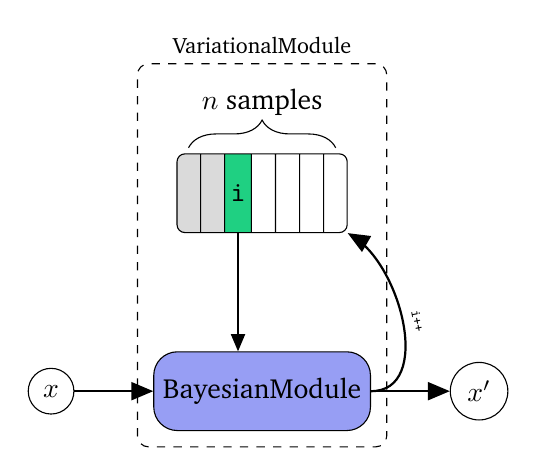
\begin{tikzpicture}[
    class/.style={rounded corners=0.3cm,minimum height=1cm,fill=blue!50,draw=black},
    other/.style={circle,draw=black},
    node distance = 1cm, 
    myrect/.style={
        draw,
        rectangle split,
        rectangle split parts=#1,
        rectangle split part align=left
        },    
    back group/.style={rounded corners, draw=black, 
                    dashed, inner xsep=0.2cm, inner ysep=0.2cm, 
                    anchor=west},
    auto
    ]
    \node[
        draw, 
        rectangle, 
        rectangle split, 
        rectangle split parts=7,
        rectangle split horizontal, 
        rectangle split part fill={
            grey,
            grey,
            brightgreen,
            white,
            white,
            white,
            white
            },
        minimum height=1cm,
        inner sep=2,
        rounded corners=0.1cm
        ] (samples) {
            \nodepart{one}
            \nodepart{two}
            \nodepart{three} \texttt{i}
            \nodepart{four}
            \nodepart{five}
            \nodepart{six}
            \nodepart{seven}
        };
    \node[class,fill=blue!50, below=1.5cm of samples] (bayesian-module) {BayesianModule};
    % \begin{scope}[on background layer]
        % \end{scope}
    \draw [->] (samples.three south) -- (bayesian-module.north -| samples.three south);
    \draw[decorate,decoration={brace, amplitude=10pt, raise=2pt}]
    (samples.one north) to node[black,midway,above=10pt] (samples-label) {$n$ samples} (samples.seven north);%
    \node (inf-modules) [back group] [fit=(bayesian-module)(samples)(samples-label),label={above:VariationalModule}]{};
    \node [other,left=of bayesian-module] (input) {$x$};
    \node [other,right=of bayesian-module] (output) {$x^\prime$};
    \draw [->,thick] (input) -- (bayesian-module);
    \draw [->,thick] (bayesian-module) -- (output);
    \draw [->,thick](bayesian-module.east) to[out=0,in=330, edge node={node [sloped,above] {\tiny \texttt{i++}}}] (samples.south east);
    \end{tikzpicture}

    \end{subfigure}
    \begin{subfigure}[b]{0.48\linewidth}
        \centering
        \caption{Implementation of \texttt{training\_step()} in \texttt{VariationalInference}.}
        % spellchecker: disable


\usetikzlibrary{shapes.multipart}
\begin{tikzpicture}
    \node[class] (model) at (0, 0) {Model};
    \node[fill=grey!50,other,below=1cm of model.south] (obs) {$\tilde{\D}$};
    \node[other,right=1.5cm of model] (loss) {$\bar{\mathcal{L}}$};

    \def\tsh{0.7cm}
    \node[minimum width=0.5cm, above=\tsh of model,anchor=center,label={above:{\tiny\texttt{training\_step()}}}] (training-step) {};

    \node[pnt] (start) at (training-step.west) {};
    \node[pnt] (end) at (training-step.east) {};
    \fill[black] (start) circle (2pt);
    \fill[black] (end) circle (2pt);
    \def\radius{1cm}

    \draw[ 
        flow,
        thick,
        postaction={decorate},
        decoration={
            markings,
            mark=at position 0.125 with {\arrow {latex}},
            mark=at position 0.375 with {\arrow {latex}},
            mark=at position 0.625 with {\arrow {latex}},
            mark=at position 0.875 with {\arrow {latex}}
        }
    ]
    (start)
    arc (90:180:\radius) node (tmp1) {}
    --
    ($(tmp1)!2.0!(tmp1 |- model)$) node[midway,anchor=center,label={left:\small{sample $n$}}] (sample-n) {}
    arc (180:270:\radius) node (tmp2) {}
    -- (tmp2 -| end) node[midway,anchor=center] (get-obs) {}
    arc (270:360:\radius) node (tmp3) {}
    -- ($(tmp3)!2.0!(tmp3 |- model)$) node[midway,anchor=center] (get-loss) {}
    arc (0:90:\radius) {}
    ;
    \def\radcirc{0.7}
    \draw[flow,thick,postaction={decorate},
        decoration={markings,
        mark=at position 0.27 with {\arrow {latex}},
        mark=at position 0.52 with {\arrow {latex}},
        mark=at position 0.77 with {\arrow {latex}}
    }]
    (get-obs.center) 
    arc (90:0:\radcirc) 
    arc (360:90:\radcirc) node[pos=0.333,anchor=north] (label) {\small repeat $n$ times}
    ;
    
    \fill[black] (sample-n) circle (2pt);
    \fill[black] (get-obs) circle (2pt);
    \fill[black] (get-loss) circle (2pt);
    
    \draw [depends] (obs) edge (model);
    \draw [depends] (model) edge (loss);
    \draw [depends] (sample-n.center) -- (model);
    


    \end{tikzpicture}

    \end{subfigure}
    \caption{Diagrams showing the implementation of variational inference.}
    \label{fig:vi-arch}
\end{figure}
If averaging over $n$ gradients, we train the model by drawing $n$ samples for every variational module of the model and then doing $n$ forward passes of the model, where each variational module keeps track of its samples.
Then, the loss is calculated for each forward pass, averaged and returned from \texttt{training\_step()}, letting Lightning handle the backward pass. 
See \cref{fig:vi-arch} for a diagram 

\subsection{MCMC Inference}
The Markov chain Monte Carlo implementation differs a bit compared to the two other implemented methods in that we need to do more with the gradients than perform an optimization step. 
It is probably possible to use PyTorch Lightning's \texttt{on\_after\_backward()} hook to implement the MCMC methods in PyTorch Lightning, however with this implementation, we instead opt to implement the sampling algorithms more explicitly.
This tactic allows for a more straightforward implementation of the samplers, which we can also use in other contexts, like directly sampling from a density function.
The different samplers are therefore implemented as  subclasses of a \texttt{Sampler} class that each define a \texttt{next\_sample()} method independently.
After initializing each sampler, we set them up by registering an object to them, defining what distribution should be sampled from. 
This object, named \texttt{Samplable}, should define the following properties: Getters and setters for the current state as a PyTorch tensor, the shape of the state, the logarithmic proportional probability density at the current state, and the corresponding gradient.  

In the context of deep learning inference, the model parameter posterior is represented by a \texttt{ParameterPosterior} object that wraps the model object and allows for the setting of different sets of observations with an \texttt{observe()} method.
This wrapper then implements the \texttt{Samplable} interface, with the state being model parameters stacked as single one-dimensional tensor, and uses the observation model and autograd to implement the remaining methods.
\begin{figure}[htbp]
    \centering
    % spellchecker: disable

\begin{tikzpicture}
    \node[class,fill=blue!50] (model) at (0, 0) {Model};
    \node[class,align=center,fill=blue!50, right=of model] (post) {Parameter-\\Posterior};
    \node[class,fill=blue!50, below=of post] (sampler) {Sampler};
    \node[other,fill=grey!50, right=3.2cm of post.center] (obs) {$\tilde{\D}$};
    \node[other,fill=red!50, right=3.2cm of sampler.center] (state) {$\theta^\ast$};
    \draw [depends] (model) -- (post);
    \draw [depends] (post) -- (sampler);
    \draw [depends] (obs) -- (post);
    \draw [depends] (sampler) -- (state);

    
    \def\yoffset{1cm}

    \node[minimum width=0, label={above:{\tiny\texttt{training\_step()}}}] 
    (start) at ($(obs)+(-0.9cm,\yoffset)$)
    {}
    ;
    
    \draw[
        thick,
        postaction={decorate},
        decoration = {
            markings,
            mark=at position 0.15 with {\arrow {latex}},
            mark=at position 0.50 with {\arrow {latex}},
            mark=at position 0.9 with {\arrow {latex}}
        }
    ] (start.center) 
    -- (obs -| start) node[inner sep=0, label={above left:{\tiny\texttt{observe()}}}] (observe) {}
    -- (state -| start) node[inner sep=0, label={above left:{\tiny\texttt{next\_sample()}}}] (next-sample) {}
    -- ($(state -| start)+(0,-\yoffset)$) node (end) {};
    ;
%     \draw[thick]
%         (start)
%         arc (90:180:\radius) node (tmp1) {}
%         -- ($(tmp1)!2.0!(tmp1 |- mid)$)
%         arc (180:270:\radius) node (tmp2) {}
%         -- (tmp2 -| end) 
%         arc (270:360:\radius) 
%         % -- ($tmp1!2.0!((obs -| tmp1)!0.5!(state -| tmp1))$)
%         ;
    % \path[name path=flow] ($(obs)+(-0.8cm,1cm)$)--($(state)+(-0.8cm,-1cm)$); 
    % \path[name path=observe] (obs)--(post); 
    % \path[name path=next] (sampler)--(state); 
    % \fill [black, name intersections={of=flow and observe}] (intersection-1) circle (2pt);
    % \fill [black, name intersections={of=flow and next}] (intersection-1) circle (2pt);
    % \path ($(obs)+(0.8cm,1cm)$) edge[draw=none] node[sloped, anchor=north] {\tiny\texttt{training\_step()}} ($(state)+(0.8cm,-1cm)$);
    % \node (a) at ($(obs)+(-0.8cm,1cm)$) {};
    % \node (b) at ($(state)+(-0.8cm,-1cm)$) {};
    \fill[black] (start) circle (2pt);
    \fill[black] (observe) circle (2pt);
    \fill[black] (next-sample) circle (2pt);
    \fill[black] (end) circle (2pt);
    % \node[red,scale=3] at (intersection of  post--obs and a--b{.};
    \end{tikzpicture}

    \caption{Basic diagram of \texttt{MCMCInference} implementation of \texttt{training\_step()} for general MCMC inference.}
    \label{fig:mcmc-arch}
\end{figure}
The MCMC inference module is thus responsible for setting up the \texttt{Samplable} wrapper with each batch of observations with \texttt{observe()}, and stepping the sampler with \texttt{next\_sample()} method. 
A diagram of the procedure can be seen in \cref{fig:mcmc-arch}.
In a particular case, when the batch size is equal to the number of elements in the whole dataset, this allows for sampling in a non-batched manner, such as with proper HMC.
This sampling strategy is not the most efficient; however, it allows for easy comparison of the different methods.

Furthermore, the module defines the additional hyperparameters, such as how many steps should be performed per sample and a burn-in period.
We define the strategy of which and how many samples we keep through the use of a \texttt{SampleContainer} object.

\section{Other Frameworks}

While independently defining the different components allows for great flexibility, it can make it cumbersome to configure and instantiate experiments, as objects may need other instantiated objects to be instantiated themselves.
As the different inference methods also need different types of objects and hyperparameters, parameterizing and documenting different configurations can become unmanageable and prone to errors.

To make experimentation as convenient as possible, we use the Hydra \autocite{yadan_hydra_2019} framework to manage the configuration for us.  
This framework allows us to specify the different configurations in terms of the \texttt{.yaml} files found in the \texttt{conf/} directory.
The configured settings can be used directly in the Python code but can also be used for object instantiation using the \texttt{\_target\_} field.
Since Hydra also supports nested instantiation.
We can instantiate just about every component of the implementation dynamically, alleviating the mentioned complexity.

This also results in the experiments being carried out using only a few scripts: \texttt{scripts/inference.py}, \texttt{scripts/sweep.py} and \texttt{scripts/sample.py}, using different sets of configuations.

With this also comes many convenient extra features such as overriding every just about anything using the command line, launching several combinations of configurations at once, and automatic management of output directory for every run.

We also use the hyperparameter optimization library Optuna \autocite{akiba_optuna_2019} for automating model fitting.
This framework is also relatively easy to implement by defining the hyperparameters of interest as the corresponding configuration fields, each specified with a search space. 
Hyperparameters are then suggested by Optuna's API and subsequently injected into the main configuration. 
The specific implementation can be seen in \texttt{scripts/sweep.py}.

\chapter{Experiments}

In the following chapters we discuss a series of experiments relating to the methods discussed above. 
We first discuss some experiments relating to improving the SGHMC through better estimation of the variance $\hat{V}$, and then perform some experiments related to the applicability of the methods in the context of deep learning, compared to more conventional methods.

\section{Estimating the variance}

In the SGHMC paper, they propose estimating the variance introduced through batching as $\hat{V}=0$, and then relying on the known simulated noise to make the inaccuracy of this estimate irrelevant. 
However, it seem to be worth investigating whether we could improve performance by providing some sort of estimate. 
This is also mentioned in the paper, however they do not seem explore the idea any further. 

Since we parameterized the upper bound $C$ with $\alpha$, we may end up with estimated noise larger than the upper bound.
Adjusting the upper bound $C$ to accommodate this, would also require adjusting the $\alpha$ parameter accordingly.
Since the $\alpha$ corresponds to the momentum decay of the algorithm, we may end up with very unstable behavior, especially for $\alpha > 1$. 
\todo[inline]{Sammenhæng mellem beta/V/B/D... skal nok rettes igennem fra teoriafdelingen af...}
Instead, we keep $\alpha=CM^{-1}$ fixed, and adjust the mass matrix $M$, implicitly adjusting $C$ as well.
With $M = M_0 W$ were $W$ is a diagonal matrix of weights, we can then, depending on the variance estimate, rescale the mass such that the upper bound $\alpha$ is sufficiently above the estimate $\hat\beta$, eg. by some factor $m_{\text{est}}$.
If we let the learning rate be given as $\eta_0$  for the unscaled mass matrix with $W = I$, then the learning rate for the scaled system can be found as $\eta = \epsilon^2 M^{-1} = \epsilon^2 M_0^{-1}W^{-1} = \eta_0 W^{-1}$, and
\begin{align*}
    m_{\text{est}} \cdot \hat{\beta}  &\leq \alpha \Leftrightarrow\\ 
    m_{\text{est}} \cdot \frac{1}{2} \hat V \eta   &\leq \alpha \Leftrightarrow\\ 
    m_{\text{est}} \cdot \frac{1}{2} \hat V \eta_0 W^{-1}  &\leq \alpha \Leftrightarrow\\ 
    m_{\text{est}} \cdot \frac{1}{2\alpha} \hat V \eta_0   &\leq W \impliedby \\
    W_{i,i} &= \begin{cases}
        1 & \frac{1}{2\alpha}m_{\text{est}} \eta_0 \hat{V}_{i,i} < 1 \\
        \frac{1}{2\alpha}m_{\text{est}} \eta_0 \hat{V}_{i,i} & \text{otherwise}
    \end{cases}
\end{align*}

The sampler then every once in a while, eg. every 50 samples, rescales the system based on the variance estimates.
If the variance estimates $\hat \beta$ happen to be greater than $\alpha$ in between the mass rescaling, the estimate is simply clamped at the upper bound $\alpha$, and no additional noise is generated.  

This method of rescaling the mass matrix is in a sense similar to the approach outlined in \cite{wenzel_how_2020}, where they also include a step calculating a preconditioning matrix, ie.
They found that using the preconditioning step generally improved performance.

There are multiple ways to go about obtaining a variance estimate.
We could try to calculate a running variance statistic using the within batch sample variance of the gradients:
\begin{equation}
    \frac{1}{|\tilde{\D}|-1}\sum_{(x_i,y_i)=\tilde{\D}} (\nabla U(\theta; x_i, y_i) - \nabla \bar{U}(\theta))^2
\end{equation}
and then scale the variance up to the fit the batch size. 
The main issue with this approach is that calculating the gradient for each observation individually within a batch is not really computationally sound.
While it may be possible to calculate the statistic above using autograd without doing a backward pass for each observation, it is trivial to do so since autograd only allows for calculating gradients of scalars. 

Instead we look at three other approaches. 
The first approach is to run through a few training batches at the start of each epoch, calculating the gradient for each batch keeping the parameters constant. 
This estimate can then be used for the remaining epoch. 
The two other approaches instead keeps track of running statistics. 
The first uses exponentially decaying running estimates of the first to moments, $m_t, v_t$ as in the ADAM algorithm \cite{kingma_adam_2017}.
Since the ADAM algorithm doesn't center the second moment estimate, the squared mean is subtracted, so that the variance is estimated as $v_t - m_t^2$.
Finally, we also try to estimate the variance as with the ADAM algorithm, however using the first moment to center the second moment estimate. 

In order to test these three different approach, they are applying to the simulated example from the previous section.
Every 10 sample, the variance of the gradient is estimated using 100 random batched from the training data set.
This estimate is then compared to the estimate.
The estimation provided by the estimators compared to the observed variance can be seen in \cref{fig:est_variances_simulated}.
\begin{figure}[htbp]
    \centering
    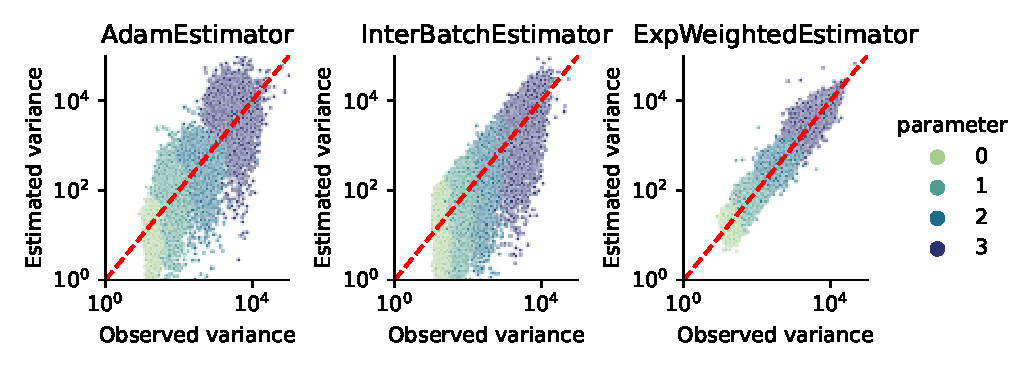
\includegraphics[width=0.9\textwidth]{Figures/simulated_sghmc_gradient_variance_estimations.pdf}
    \caption{Estimated variance compared to observed variances}
    \label{fig:est_variances_simulated}
\end{figure}
\begin{table}[htbp]
    \centering
    \begin{tabular}{lrrrr}
\toprule
parameter &    0 &    1 &    2 &    3 \\
variance\_estimator   &      &      &      &      \\
\midrule
AdamEstimator        & 0.65 & 2.03 & 1.67 & 2.98 \\
ConstantEstimator    & 1.00 & 1.00 & 1.00 & 1.00 \\
ExpWeightedEstimator & 0.30 & 0.41 & 0.42 & 0.49 \\
InterBatchEstimator  & 1.00 & 0.98 & 0.98 & 0.94 \\
\bottomrule
\end{tabular}

    \caption{Relative errors for the different estimation schemes,}
\end{table}
Note that these values are plot using a logarithmic scale, so the estimates may seem better than they actually are, especially with when it comes to overestimating. 
It may still be that they are better than simply setting $\hat\beta=0$ in terms of estimating the posterior correctly.
In \cref{fig:simualted_var_est_joint_comp}, the sampled marginal distribution of $a_1$ and $a_3$ are shown again, now compared SGHMC with and without a variance estimator.
\begin{figure}[htbp]
    \centering
    \begin{subfigure}[t]{0.4\textwidth}
        \centering
        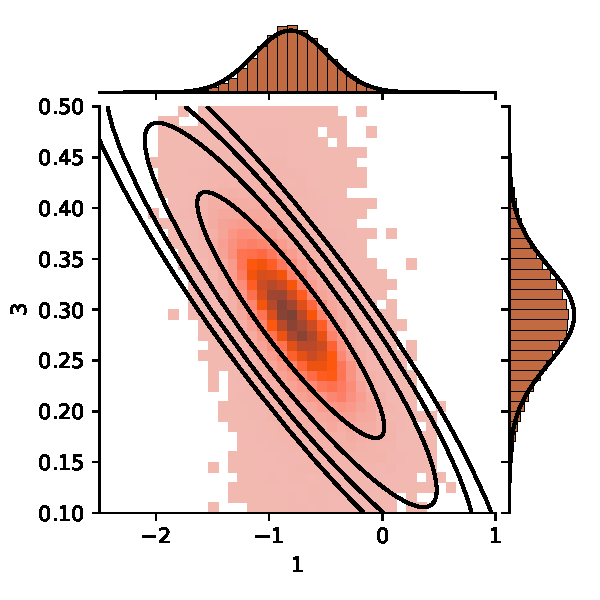
\includegraphics[width=\textwidth]{Figures/simulated_joint_SGHMC_5.pdf} 
        \caption{SGHMC with with gradient variance estimated as $\hat{V}=0$.}
    \end{subfigure}
    \begin{subfigure}[t]{0.4\textwidth}
        \centering
        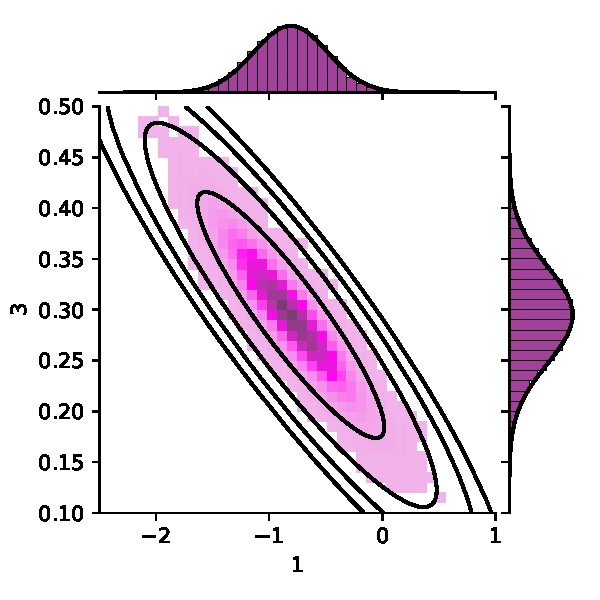
\includegraphics[width=\textwidth]{Figures/simulated_joint_SGHMCWithVarianceEstimator_5.pdf} 
        \caption{SGHMC with using the exponentially scaled estimator of gradient variance}
    \end{subfigure}
    \caption{Joint distribution of samples for $a_1$ and $a_3$ for the polynomial regression example for HMC and SGHMC for different batch sizes, with the actual posterior density also shown.}
    \label{fig:simualted_var_est_joint_comp}
\end{figure}
In this case, it does indeed seem like estimating the variance is helping the sampler.
This may come down to the approach with estimated variance is able to adjust the step size down, lowering discretization and batch error compared to SGHMC without an estimator. 

\subsection{Marginal distribution of momentum}

In \cite{wenzel_how_2020}, they propose using the marginal distribution of the momentum as a test of the sampling assumptions. 
Per the dynamical system, if the system is simulated exactly, the marginal distribution of $r$ should be $\mathcal{N}(0, M)$. 
We should therefore have that $r M^{-1/2} \sim \mathcal{N}(0, 1)$. 
Applying the inner product, $r^T M r$ should therefore follow a $\chi^2(d)$ distribution, where $d$ is the length of $r$. 
If we look at some $c$ quantile of the $\chi^2(d)$ distribution, we would expect a fraction $c$ of the samples for $r^T M r$ to land within that particular quantile. 
To this end, let $\hat T_{0.99}$ be the fraction of samples for some set of $d$ parameters, that fall within a $0.99$ quantile of the $\chi^2(d)$ distribution. 
We should therefore expect $\hat T_{0.99}=0.99$ given a perfectly simulated system.
This allows us to test the correctness of our sampler, even if we don't know the true posterior, which is going to be the case in the following experiments.

Applying this statistic, we can see whether the estimation of the variance helps with regard to the correctness of the simulation. 
Returning back to our simulated polynomial example, in the previous experiment, the momentum were resampled every $10$ epochs, to make to comparison to regular HMC as clear as possible. 
However, if we resample the momentum from the marginal distribution too often, the $\hat{T}_{0.99}$ measure would obviously be less informative with regard to the influence of discretization and batching error. 
The momentum is therefore instead resampled every $1000$ steps, with a slightly lower learning rate of $\eta=4 \cdot 10^{-5}$.
The lower learning rate is used since otherwise, the SGHMC sampler with $\hat{\beta}=0$ becomes unstable. 
\begin{figure}[htb]
    \centering
    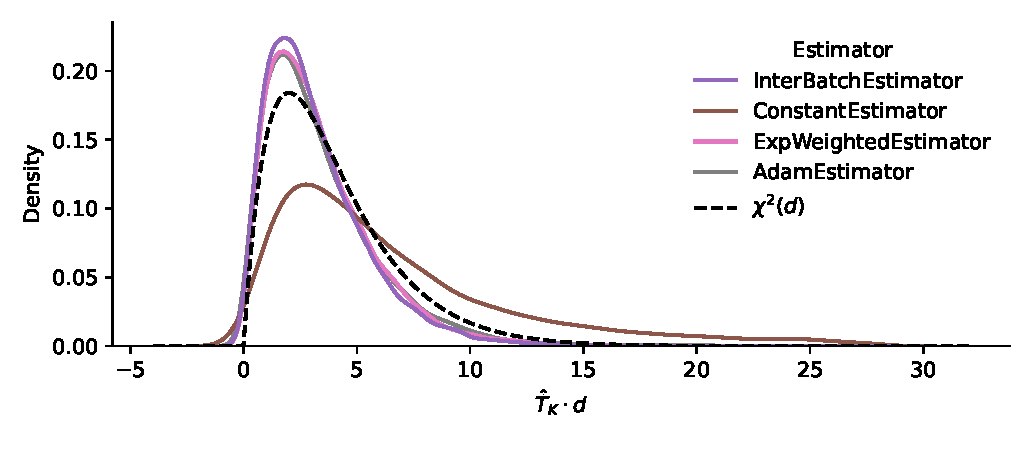
\includegraphics[width=0.9\textwidth]{Figures/temperature_sum_chi2_comp.pdf}
    \caption{<caption>}
    \label{fig:temperature_sum_chi2_comp}
\end{figure}
\begin{table}[htb]
    \centering
    \begin{tabular}{lrr}
\toprule
{} &    frac\_in\_99 &        pm \\
parameter & \multicolumn{2}{l}{linear.weight} \\
variance\_estimator   &               &           \\
\midrule
AdamEstimator        &      0.992099 &  0.001363 \\
ConstantEstimator    &      0.835864 &  0.005704 \\
ExpWeightedEstimator &      0.996358 &  0.000928 \\
InterBatchEstimator  &      0.995617 &  0.001017 \\
\bottomrule
\end{tabular}

    \caption{<caption>}
    \label{tbl:temp_99}
\end{table}
The resulting distribution of $r^T M r$ can be seen in \cref{fig:temperature_sum_chi2_comp}, compared against the expected $\chi^2$ distribution. 
We see that the while the samplers with estimated variance doesn't fit the distributional assumptions, they are all much closer than the for the sampler with $\hat \beta = 0$.
The $\hat T_{0.99}$ statistic have also been calculated in \cref{tbl:temp_99}, alongside a confidence interval based on the binomial distribution.

\todo[inline]{prøv med mindre stepsize eller kom videre? Mest for at vise om varians estimation kunne afhælpe fx dårlig lr eller beta estimat. (hvilket det kunne, til dels?)}

It seem like the samplers with estimated variance are all underdispersing slightly, compared to the actual posterior. with  which would make sense if we are overestimating variance.
Looking at the PLOT, the estimation margin estimates also seems relatively uniformly distributed on the log scale, which would mean that we are generally overestimating with larger magnitude. 
Since we are overestimating the noise from batching, this would lead to us not adding sufficient noise to the system, leading to underdispersion.

\section{MNIST}
In this section, we will explore the performance of the different methods on the MNIST dataset for classification.

While the original SGHMC paper does explore the performance on the MNIST dataset compared to dropout, they do so with a feed forward neural network with only a single hidden layer of size 100.


While they demonstrate comparable performance, it doesn't really serve to compare the performance of the methods with respect to deep learning with  

While the MNIST dataset is not really 

\begin{figure}[htbp]
    \centering
    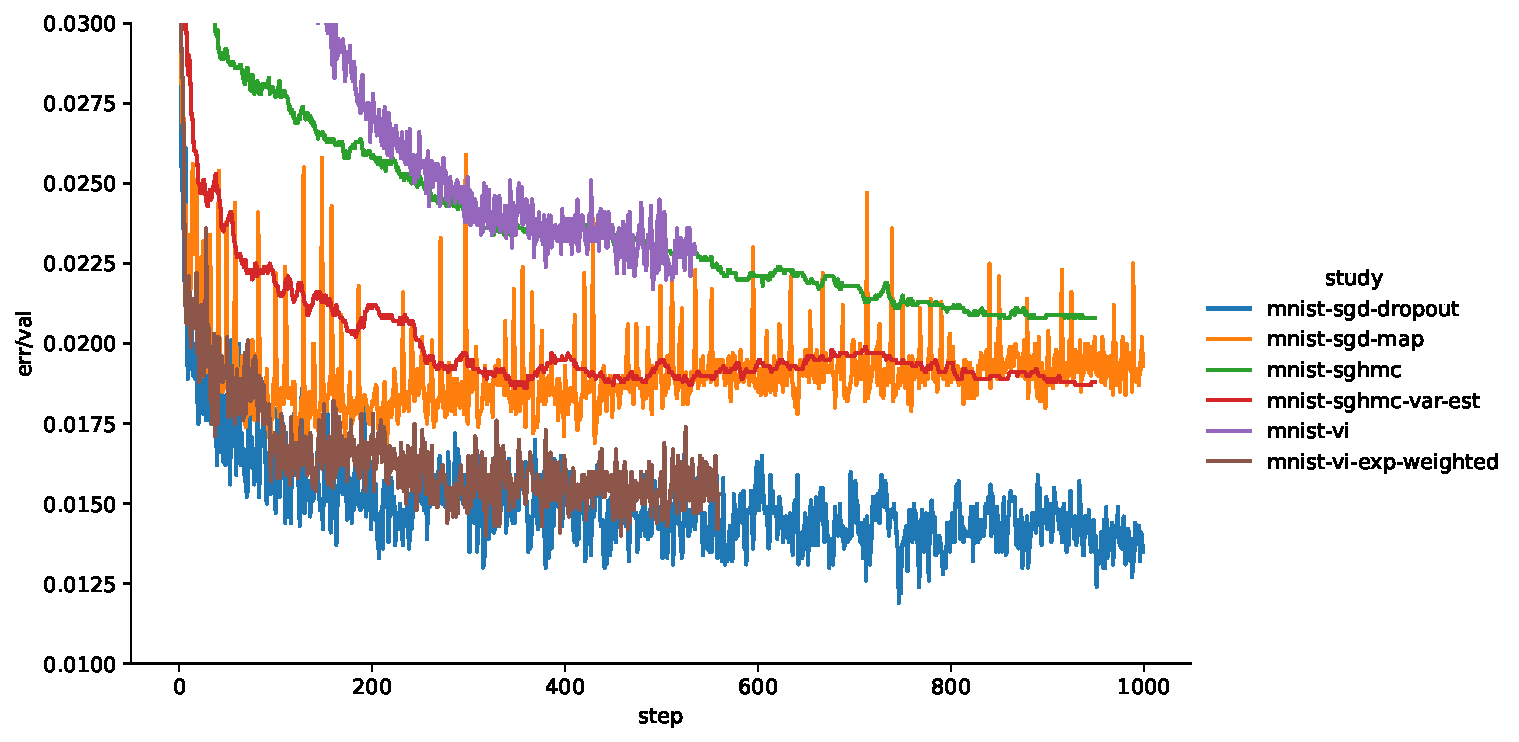
\includegraphics[width=.9\linewidth]{Figures/mnist-best-runs-val-curves.pdf}
    \caption{Validation curves for best run found during hyperparameter search.}
    \label{<label>}
\end{figure}

\section{Convolutional Neural Net}

\subsection{CIFAR10}

\subsection{Densenet}




\chapter{Conlusion}

\section{Conclusion}
We can get some(?) or not? improvement with respect to uncertianty estimation.

one stop shop for all mean

performance?

estimatino variance helps?


\section{Discussion}
Applicability of mcmc methods for non-deep learning with lots of data -> registerforskning fx.

what does it even mean to have a prior. correcntness of model

Reweightnig/resmapling of samplesaccording to validation.

how much does the correctness of the model matter -> model is obv. wrong...

various problems with hparam search approach
But prabably relavent for wanting to fit a model given a finitiate evalition budget
all seem to be overfitting <- fine in the sense that we dont want to continue training. However probably is biased towards qui

identificability huge search spaces

discuss implementation
 - Robust -- currently adhoc blablabla


ineteristing to train from scratch? smaller models worked fine -> batch norm... proably doesnt do muich for smaller models compared to deep models
-> dirty likelihoods


VI methods -> flows?
bunch of other stuff we could try to improve the performance of any of the methods lr scheduling, feature engineering, other model structures etc. 
dropout for prob method per dirty likelihood.

lack of modelling techniques?

%%%%%%%%%%%%%

\nocite{*}
\printbibliography[heading=bibintoc,title={Bibliography}]
\cleardoublepage 
\appendix
\chapter{Hyperparameter sweeps} 

\section{MNIST} \label{apx:mnist-sweep}
\begin{table}[H]
    \centering
    \resizebox{
        \ifdim\width>\columnwidth
        \columnwidth
      \else
        \width
      \fi
    }{!}{\small
    \begin{tabular}{lp{2.3cm}p{2.3cm}p{2.3cm}}
\toprule
{} &  val. error &         \texttt{lr} &  \texttt{dropout} \\
trial &             &                     &                   \\
\midrule
19    &      0.0135 & $4.87\times10^{-4}$ &          0.289191 \\
16    &      0.0139 & $9.74\times10^{-4}$ &          0.281853 \\
21    &      0.0139 & $3.60\times10^{-4}$ &          0.299949 \\
14    &      0.0139 & $9.74\times10^{-4}$ &          0.288437 \\
8     &      0.0143 & $2.61\times10^{-4}$ &          0.520788 \\
13    &      0.0143 & $1.57\times10^{-4}$ &          0.441916 \\
11    &      0.0146 & $3.24\times10^{-4}$ &          0.397340 \\
4     &      0.0146 & $1.59\times10^{-4}$ &          0.437008 \\
15    &      0.0146 & $7.52\times10^{-4}$ &          0.324764 \\
17    &      0.0148 & $7.13\times10^{-4}$ &          0.263096 \\
\bottomrule
\end{tabular}

    }
    \caption{Top 10 hyperparameters for SGD with dropout according to optuna sweep.}
    \label{tab:mnist-sgd-dropout-hparams}
\end{table}


\begin{table}[H]
    \centering
    \resizebox{
        \ifdim\width>\columnwidth
        \columnwidth
      \else
        \width
      \fi
    }{!}{\small
    \begin{tabular}{lp{2.3cm}p{2.3cm}p{2.3cm}p{2.3cm}p{2.3cm}}
\toprule
{} &  Val. error &         \texttt{lr} &  \texttt{log\_sigma\_1} &  \texttt{log\_sigma\_2} &  \texttt{mixture\_ratio} \\
trial &             &                     &                         &                         &                          \\
\midrule
15    &      0.0193 & $3.92\times10^{-4}$ &                       0 &                      -7 &                 0.704007 \\
2     &      0.0202 & $8.71\times10^{-5}$ &                       0 &                      -6 &                 0.643522 \\
5     &      0.0202 & $2.66\times10^{-5}$ &                       0 &                      -8 &                 0.524438 \\
1     &      0.0207 & $7.55\times10^{-5}$ &                       0 &                      -8 &                 0.283183 \\
10    &      0.0207 & $1.32\times10^{-4}$ &                       0 &                      -6 &                 0.562885 \\
11    &      0.0209 & $1.53\times10^{-5}$ &                       0 &                      -8 &                 0.496544 \\
6     &      0.0211 & $6.19\times10^{-4}$ &                      -1 &                      -6 &                 0.640225 \\
12    &      0.0211 & $6.83\times10^{-5}$ &                       0 &                      -8 &                 0.700414 \\
13    &      0.0211 & $3.76\times10^{-5}$ &                       0 &                      -6 &                 0.654232 \\
8     &      0.0213 & $2.59\times10^{-4}$ &                      -1 &                      -6 &                 0.400428 \\
\bottomrule
\end{tabular}

    }
    \caption{Top 10 hyperparameters for sgd with MAP estimate according to optuna sweep.}
    \label{tab:mnist-sgd-map-hparams}
\end{table}



\begin{table}[H]
    \centering
    \resizebox{
        \ifdim\width>\columnwidth
        \columnwidth
      \else
        \width
      \fi
    }{!}{\small
    \begin{tabular}{lp{2.3cm}p{2.3cm}p{2.3cm}p{2.3cm}}
\toprule
{} &  val. error &  \texttt{alpha} &         \texttt{lr} &  \texttt{resample\_momentum\_every} \\
trial &             &                 &                     &                                     \\
\midrule
53    &      0.0208 &        0.063935 & $1.47\times10^{-6}$ &                               95562 \\
18    &      0.0209 &        0.011664 & $1.39\times10^{-7}$ &                               82773 \\
36    &      0.0209 &        0.039170 & $9.97\times10^{-7}$ &                               55108 \\
4     &      0.0209 &        0.004083 & $1.57\times10^{-7}$ &                               88291 \\
41    &      0.0210 &        0.017220 & $6.38\times10^{-7}$ &                               23433 \\
26    &      0.0210 &        0.004822 & $9.79\times10^{-8}$ &                               91410 \\
22    &      0.0210 &        0.064860 & $1.25\times10^{-6}$ &                               95925 \\
3     &      0.0210 &        0.066075 & $1.29\times10^{-6}$ &                               58285 \\
32    &      0.0210 &        0.003841 & $1.07\times10^{-7}$ &                               20313 \\
44    &      0.0211 &        0.002584 & $1.28\times10^{-7}$ &                                 615 \\
\bottomrule
\end{tabular}

    }
    \caption{Top 10 hyperparameters for SGHMC according to optuna sweep.}
    \label{tab:mnist-sghmc-hparams}
\end{table}


\begin{table}[H]
    \centering
    \resizebox{
        \ifdim\width>\columnwidth
        \columnwidth
      \else
        \width
      \fi
    }{!}{\small
    \begin{tabular}{lp{2.3cm}p{2.3cm}p{2.3cm}p{2.3cm}p{2.3cm}}
\toprule
{} &  val. error &  \texttt{alpha} &  \texttt{estimation\_margin} &         \texttt{lr} &  \texttt{resample\_momentum\_every} \\
trial &             &                 &                              &                     &                                     \\
\midrule
27    &      0.0188 &        0.003067 &                    12.371372 & $1.46\times10^{-7}$ &                               84178 \\
32    &      0.0192 &        0.003452 &                    23.745188 & $6.14\times10^{-8}$ &                               13723 \\
23    &      0.0195 &        0.002886 &                    20.353818 & $5.54\times10^{-8}$ &                               66410 \\
22    &      0.0195 &        0.001037 &                    11.514889 & $2.42\times10^{-8}$ &                               68272 \\
21    &      0.0197 &        0.001069 &                    15.986332 & $2.18\times10^{-8}$ &                               38094 \\
48    &      0.0200 &        0.001215 &                     9.422489 & $4.10\times10^{-8}$ &                               41127 \\
52    &      0.0206 &        0.001755 &                    12.920221 & $4.10\times10^{-8}$ &                               26360 \\
53    &      0.0212 &        0.001228 &                     8.842851 & $2.38\times10^{-8}$ &                               21035 \\
33    &      0.0212 &        0.004063 &                    16.947506 & $1.04\times10^{-7}$ &                               88210 \\
44    &      0.0213 &        0.001278 &                    19.633689 & $2.68\times10^{-8}$ &                               13024 \\
\bottomrule
\end{tabular}

    }
    \caption{Top 10 hyperparameters for SGHMC with variance estimation according to optuna sweep.}
    \label{tab:mnist-sghmc-var-est-hparams}
\end{table}



\begin{table}[H]
    \centering
    \resizebox{
        \ifdim\width>\columnwidth
        \columnwidth
      \else
        \width
      \fi
    }{!}{\small
    \begin{tabular}{lp{2cm}p{2cm}p{2cm}p{2cm}p{2cm}p{2cm}}
\toprule
{} &  val. error &         \texttt{lr} &  \texttt{n\_particles} &  \texttt{log\_sigma\_1} &  \texttt{log\_sigma\_2} &  \texttt{mixture\_ratio} \\
trial &             &                     &                        &                         &                         &                          \\
\midrule
13    &      0.0219 & $4.88\times10^{-4}$ &                      7 &                       0 &                      -7 &                 0.469902 \\
12    &      0.0224 & $1.53\times10^{-4}$ &                      6 &                       0 &                      -7 &                 0.474150 \\
4     &      0.0228 & $9.95\times10^{-5}$ &                      5 &                       0 &                      -7 &                 0.513909 \\
10    &      0.0229 & $4.68\times10^{-5}$ &                      8 &                       0 &                      -7 &                 0.600455 \\
7     &      0.0240 & $1.28\times10^{-4}$ &                      3 &                       0 &                      -7 &                 0.286113 \\
3     &      0.0244 & $1.33\times10^{-5}$ &                      7 &                      -1 &                      -7 &                 0.374102 \\
14    &      0.0252 & $6.46\times10^{-4}$ &                     10 &                       0 &                      -7 &                 0.355078 \\
8     &      0.0270 & $9.12\times10^{-4}$ &                      5 &                      -1 &                      -6 &                 0.617132 \\
9     &      0.0274 & $4.93\times10^{-4}$ &                      5 &                      -1 &                      -6 &                 0.367210 \\
6     &      0.0277 & $3.65\times10^{-4}$ &                      6 &                      -1 &                      -6 &                 0.621738 \\
\bottomrule
\end{tabular}

    }
    \caption{Top 10 hyperparameters for variational inference according to optuna sweep.}
    \label{tab:mnist-vi-hparams}
\end{table}


\begin{table}[H]
    \centering
    \resizebox{
        \ifdim\width>\columnwidth
        \columnwidth
      \else
        \width
      \fi
    }{!}{\small
    \begin{tabular}{lp{2.3cm}p{2.3cm}p{2.3cm}p{2.3cm}p{2.3cm}p{2.3cm}}
\toprule
{} &  val. error &         \texttt{lr} &  \texttt{n\_particles} &  \texttt{log\_sigma\_1} &  \texttt{log\_sigma\_2} &  \texttt{mixture\_ratio} \\
trial &             &                     &                        &                         &                         &                          \\
\midrule
10    &      0.0153 & $6.59\times10^{-4}$ &                      9 &                       0 &                      -7 &                 0.536381 \\
0     &      0.0169 & $8.61\times10^{-4}$ &                      9 &                       0 &                      -7 &                 0.513667 \\
1     &      0.0193 & $1.24\times10^{-4}$ &                      9 &                      -1 &                      -8 &                 0.254852 \\
5     &      0.0209 & $3.34\times10^{-5}$ &                      7 &                       0 &                      -8 &                 0.349681 \\
7     &      0.0216 & $5.88\times10^{-5}$ &                      9 &                      -1 &                      -7 &                 0.433288 \\
4     &      0.0228 & $1.83\times10^{-4}$ &                      3 &                       0 &                      -6 &                 0.715279 \\
8     &      0.0243 & $2.30\times10^{-4}$ &                      5 &                      -2 &                      -8 &                 0.637049 \\
2     &      0.0251 & $9.24\times10^{-5}$ &                      7 &                      -2 &                      -7 &                 0.653505 \\
9     &      0.0253 & $5.50\times10^{-5}$ &                      1 &                      -2 &                      -8 &                 0.285662 \\
3     &      0.0272 & $1.86\times10^{-4}$ &                      9 &                      -2 &                      -7 &                 0.317423 \\
\bottomrule
\end{tabular}

    }
    \caption{Top 10 hyperparameters for VI with exponentially scaled KL-term according to optuna sweep.}
    \label{tab:mnist-vi-exp-weighted-hparams}
\end{table}



\begin{table}[H]
    \centering
    \begin{tabular}{p{4cm}p{9cm}}
        \toprule
        Algorithm & Parameters chosen \\ \midrule
        SGD (dropout) & $\texttt{lr}=5\times 10^{-4}$,
        $\texttt{dropout}=0.3$ \\ \midrule
        SGD (MAP) & 
        $\texttt{lr}=4 \times 10^{-4}$, 
        $\log\sigma_1=0$, 
        $\log\sigma_2=-7$, 
        $\texttt{mixture\_ratio}=0.7$ \\ \midrule
        SGHMC & $\texttt{lr}=10^{-6}$, $\alpha=0.05$ \\ \midrule
        SGHMC (with variance estimate) &  $\texttt{lr}= 5 \times 10^{-8}$, 
        $\alpha=0.003$,
        $\texttt{estimation\_margin}=20$ \\ 
        Variational inference &    
        $\texttt{lr}=4 \times 10^{-4}$,
        $\log\sigma_1=0$,
        $\log\sigma_2=-7$,
        $\texttt{mixture\_ratio}=0.4$,
        $\texttt{n\_particles}=8$ \\
        \bottomrule
    \end{tabular}
    \caption{Chosen hyperparameters for MNIST.}
    \label{tab:mnist-hparams}
\end{table}

\FloatBarrier

\section{CIFAR10 - Small model}

\begin{table}[H]
    \centering
    \resizebox{
        \ifdim\width>\columnwidth
        \columnwidth
      \else
        \width
      \fi
    }{!}{\small
    \begin{tabular}{lp{2.3cm}p{2.3cm}p{2.3cm}p{2.3cm}p{2.3cm}}
\toprule
{} &  val. error &         \texttt{lr} &  \texttt{log\_sigma\_1} &  \texttt{log\_sigma\_2} &  \texttt{mixture\_ratio} \\
trial &             &                     &                         &                         &                          \\
\midrule
34    &      0.2713 & $8.38\times10^{-4}$ &                      -2 &                      -8 &                 0.518845 \\
26    &      0.2732 & $9.52\times10^{-4}$ &                      -2 &                      -8 &                 0.584126 \\
36    &      0.2734 & $9.05\times10^{-4}$ &                      -2 &                      -8 &                 0.622803 \\
27    &      0.2735 & $8.08\times10^{-4}$ &                      -2 &                      -8 &                 0.622519 \\
29    &      0.2737 & $7.34\times10^{-4}$ &                      -2 &                      -8 &                 0.702049 \\
37    &      0.2759 & $7.64\times10^{-4}$ &                      -2 &                      -8 &                 0.555411 \\
21    &      0.2760 & $8.75\times10^{-4}$ &                      -2 &                      -8 &                 0.527001 \\
25    &      0.2781 & $9.69\times10^{-4}$ &                      -2 &                      -8 &                 0.584764 \\
22    &      0.2784 & $3.03\times10^{-4}$ &                      -2 &                      -8 &                 0.564640 \\
15    &      0.2785 & $5.35\times10^{-4}$ &                      -2 &                      -8 &                 0.430976 \\
\bottomrule
\end{tabular}

    }
    \caption{Top 10 hyperparameters for SGD (MAP) on CIFAR10 dataset according to optuna sweep.}
    \label{tab:cifar-small-sgd-map-hparams}
\end{table}

\begin{table}[H]
    \centering
    \resizebox{
        \ifdim\width>\columnwidth
        \columnwidth
      \else
        \width
      \fi
    }{!}{\small
    \begin{tabular}{lp{2.3cm}p{2.3cm}p{2.3cm}}
\toprule
{} &  val. error &         \texttt{lr} &  \texttt{dropout} \\
trial &             &                     &                   \\
\midrule
113   &      0.2914 & $2.56\times10^{-4}$ &          0.592670 \\
33    &      0.2936 & $2.21\times10^{-4}$ &          0.622964 \\
43    &      0.2938 & $5.14\times10^{-4}$ &          0.568866 \\
97    &      0.2949 & $4.42\times10^{-4}$ &          0.581561 \\
123   &      0.2951 & $2.63\times10^{-4}$ &          0.556047 \\
80    &      0.2952 & $2.79\times10^{-4}$ &          0.662944 \\
65    &      0.2954 & $4.69\times10^{-4}$ &          0.604625 \\
99    &      0.2954 & $3.03\times10^{-4}$ &          0.579064 \\
56    &      0.2957 & $5.45\times10^{-4}$ &          0.530754 \\
105   &      0.2958 & $3.15\times10^{-4}$ &          0.562173 \\
\bottomrule
\end{tabular}

    }
    \caption{Top 10 hyperparameters for SGD (dropout) on CIFAR10 dataset according to optuna sweep.}
    \label{tab:cifar-small-sgd-dropout-hparams}
\end{table}

\begin{table}[H]
    \centering
    \resizebox{
        \ifdim\width>\columnwidth
        \columnwidth
      \else
        \width
      \fi
    }{!}{\small
    \begin{tabular}{lp{2.3cm}p{2.3cm}p{2.3cm}p{2.3cm}}
\toprule
{} &  val. error &  \texttt{alpha} &         \texttt{lr} &  \texttt{resample\_momentum\_every} \\
trial &             &                 &                     &                                     \\
\midrule
17    &      0.2178 &        0.061482 & $9.37\times10^{-8}$ &                                4901 \\
41    &      0.2192 &        0.042806 & $5.82\times10^{-8}$ &                                4440 \\
18    &      0.2249 &        0.140438 & $9.80\times10^{-8}$ &                               11682 \\
19    &      0.2253 &        0.189957 & $2.24\times10^{-7}$ &                               67277 \\
28    &      0.2255 &        0.050460 & $9.14\times10^{-8}$ &                                2257 \\
35    &      0.2292 &        0.051872 & $6.54\times10^{-8}$ &                                7179 \\
24    &      0.2322 &        0.017190 & $7.30\times10^{-8}$ &                               15118 \\
38    &      0.2348 &        0.185612 & $1.08\times10^{-7}$ &                                2032 \\
16    &      0.2355 &        0.138670 & $2.60\times10^{-7}$ &                                1055 \\
33    &      0.2357 &        0.052567 & $1.17\times10^{-7}$ &                                2165 \\
\bottomrule
\end{tabular}

    }
    \caption{Top 10 hyperparameters for SGHMC on CIFAR10 dataset according to optuna sweep.}
    \label{tab:cifar-small-sghmc-hparams}
\end{table}

\begin{table}[H]
    \centering
    \resizebox{
        \ifdim\width>\columnwidth
        \columnwidth
      \else
        \width
      \fi
    }{!}{\small
    \begin{tabular}{lp{2.3cm}p{2.3cm}p{2.3cm}p{2.3cm}p{2.3cm}}
\toprule
{} &  val. error &  \texttt{alpha} &  \texttt{estimation\_margin} &         \texttt{lr} &  \texttt{resample\_momentum\_every} \\
trial &             &                 &                              &                     &                                     \\
\midrule
10    &      0.2433 &        0.054908 &                     1.689164 & $2.47\times10^{-8}$ &                                 899 \\
6     &      0.2460 &        0.080571 &                     4.715426 & $6.05\times10^{-8}$ &                                 247 \\
15    &      0.2461 &        0.035738 &                     2.138436 & $9.45\times10^{-8}$ &                                3569 \\
25    &      0.2468 &        0.120272 &                     3.218168 & $5.71\times10^{-8}$ &                                2993 \\
18    &      0.2512 &        0.069275 &                     2.870169 & $5.49\times10^{-8}$ &                                 168 \\
17    &      0.2542 &        0.015561 &                     2.570056 & $6.52\times10^{-8}$ &                                 501 \\
22    &      0.2559 &        0.041594 &                     1.697501 & $7.66\times10^{-8}$ &                               27677 \\
8     &      0.2560 &        0.005212 &                     2.386055 & $1.14\times10^{-8}$ &                               41194 \\
21    &      0.2621 &        0.065089 &                     2.276452 & $1.78\times10^{-7}$ &                                2465 \\
23    &      0.2626 &        0.025060 &                     3.154796 & $3.59\times10^{-8}$ &                                2521 \\
\bottomrule
\end{tabular}

    }
    \caption{Top 10 hyperparameters for SGHMC (with var. est.) on CIFAR10 dataset according to optuna sweep.}
    \label{tab:cifar-small-sghmc-var-est-hparams}
\end{table}

\begin{table}[H]
    \centering
    \resizebox{
        \ifdim\width>\columnwidth
        \columnwidth
      \else
        \width
      \fi
    }{!}{\small
    \begin{tabular}{lp{2.3cm}p{2.3cm}p{2.3cm}p{2.3cm}p{2.3cm}p{2.3cm}}
\toprule
{} &  val. error &         \texttt{lr} &  \texttt{n\_particles} &  \texttt{log\_sigma\_1} &  \texttt{log\_sigma\_2} &  \texttt{mixture\_ratio} \\
trial &             &                     &                        &                         &                         &                          \\
\midrule
17    &      0.2747 & $7.54\times10^{-4}$ &                     10 &                      -1 &                      -8 &                 0.332619 \\
15    &      0.2772 & $6.75\times10^{-4}$ &                     10 &                       0 &                      -8 &                 0.336076 \\
18    &      0.2776 & $5.66\times10^{-4}$ &                     10 &                      -1 &                      -8 &                 0.471768 \\
21    &      0.2782 & $8.00\times10^{-4}$ &                     10 &                      -1 &                      -8 &                 0.477761 \\
16    &      0.2807 & $5.68\times10^{-4}$ &                     10 &                       0 &                      -8 &                 0.250722 \\
22    &      0.2835 & $5.26\times10^{-4}$ &                     10 &                      -2 &                      -8 &                 0.264284 \\
31    &      0.2837 & $8.95\times10^{-4}$ &                     10 &                      -1 &                      -8 &                 0.481262 \\
36    &      0.2838 & $4.56\times10^{-4}$ &                      8 &                      -1 &                      -8 &                 0.490509 \\
24    &      0.2866 & $9.08\times10^{-4}$ &                      9 &                      -1 &                      -8 &                 0.343383 \\
30    &      0.2872 & $9.76\times10^{-4}$ &                     10 &                       0 &                      -8 &                 0.473087 \\
\bottomrule
\end{tabular}

    }
    \caption{Top 10 hyperparameters for VI on CIFAR10 dataset according to optuna sweep.}
    \label{tab:cifar-small-vi-hparams}
\end{table}

\begin{table}[H]
    \centering
    \resizebox{
        \ifdim\width>\columnwidth
        \columnwidth
      \else
        \width
      \fi
    }{!}{\small
    \begin{tabular}{lp{2.3cm}p{2.3cm}p{2.3cm}p{2.3cm}p{2.3cm}p{2.3cm}}
\toprule
{} &  val. error &         \texttt{lr} &  \texttt{n\_particles} &  \texttt{log\_sigma\_1} &  \texttt{log\_sigma\_2} &  \texttt{mixture\_ratio} \\
trial &             &                     &                        &                         &                         &                          \\
\midrule
3     &      0.2269 & $8.70\times10^{-4}$ &                      7 &                      -2 &                      -8 &                 0.493947 \\
10    &      0.2323 & $9.02\times10^{-4}$ &                      4 &                      -2 &                      -8 &                 0.327203 \\
11    &      0.2339 & $8.25\times10^{-4}$ &                      4 &                      -2 &                      -8 &                 0.324477 \\
12    &      0.2410 & $9.53\times10^{-4}$ &                      9 &                      -2 &                      -8 &                 0.475304 \\
5     &      0.2578 & $2.64\times10^{-4}$ &                      4 &                      -2 &                      -7 &                 0.610316 \\
4     &      0.2778 & $1.74\times10^{-4}$ &                      8 &                      -1 &                      -7 &                 0.692732 \\
1     &      0.2794 & $6.79\times10^{-5}$ &                      8 &                       0 &                      -8 &                 0.410514 \\
13    &      0.2818 & $6.64\times10^{-4}$ &                      1 &                      -2 &                      -7 &                 0.365220 \\
14    &      0.2850 & $9.16\times10^{-4}$ &                      5 &                      -1 &                      -8 &                 0.512017 \\
7     &      0.2888 & $6.50\times10^{-4}$ &                      2 &                       0 &                      -7 &                 0.532149 \\
\bottomrule
\end{tabular}

    }
    \caption{Top 10 hyperparameters for VI (exp. KL weight) on CIFAR10 dataset according to optuna sweep.}
    \label{tab:cifar-small-vi-exp-weighted-hparams}
\end{table}


\cleartoleftpage
\newgeometry{left=28mm,right=14mm,top=42mm,bottom=14mm}
\thispagestyle{empty}
\pagecolor{frontbackcolor}
\color{white}

% \blindtext % Remove this for a blank page or write your own text

\vspace*{\fill}



\begin{tabular}{@{}l}
    Technical \\ 
    University of \\ 
    Denmark \\
    \\
    \addressI \\
    \addressII \\
    Tlf. 4525 1700 \\
    \\
    \url{\departmentwebsite}
\end{tabular}



\end{document}